% !TeX encoding = UTF-8
% !TeX program = xelatex
% !TeX spellcheck = en_US

\documentclass[degree=bachelor]{thuthesis}
  % 学位 degree:
  %   doctor | master | bachelor | postdoc
  % 学位类型 degree-type:
  %   academic(默认)| professional


% 论文基本配置,加载宏包等全局配置
% !TeX root = ../main.tex

% 论文基本信息配置

\thusetup{
  %******************************
  % 注意:
  %   1. 配置里面不要出现空行
  %   2. 不需要的配置信息可以删除
  %******************************
  %
  % 标题
  %   可使用“\\”命令手动控制换行
  %
  title  = {基于手机传感的任意桌面文本输入技术研究},
  title* = {Technical Research of Text Entry on Any Table Based on Phone Sensors},
  %
  % 学位
  %   1. 学术型
  %      - 中文
  %        需注明所属的学科门类,例如:
  %        哲学、经济学、法学、教育学、文学、历史学、理学、工学、农学、医学、
  %        军事学、管理学、艺术学
  %      - 英文
  %        博士:Doctor of Philosophy
  %        硕士:
  %          哲学、文学、历史学、法学、教育学、艺术学门类,公共管理学科
  %          填写“Master of Arts“,其它填写“Master of Science”
  %   2. 专业型
  %      直接填写专业学位的名称,例如:
  %      教育博士、工程硕士等
  %      Doctor of Education, Master of Engineering
  %   3. 本科生不需要填写
  %
%   degree-name  = {工学硕士},
%   degree-name* = {Master of Science},
  %
  % 培养单位
  %   填写所属院系的全名
  %
  department = {计算机科学与技术系},
  %
  % 学科
  %   1. 学术型学位
  %      获得一级学科授权的学科填写一级学科名称,其他填写二级学科名称
  %   2. 工程硕士
  %      工程领域名称
  %   3. 其他专业型学位
  %      不填写此项
  %   4. 本科生不需要填写
  %
  discipline  = {计算机科学与技术},
  discipline* = {Computer Science and Technology},
  %
  % 姓名
  %
  author  = {王琛},
  author* = {Wang Chen},
  %
  % 指导教师
  %   中文姓名和职称之间以英文逗号“,”分开,下同
  %
  supervisor  = {易鑫助理研究员},
  supervisor* = {Professor Tao Pin},
  %
  % 副指导教师
  %
%   associate-supervisor  = {易鑫},
%   associate-supervisor* = {},
  %
  % 联合指导教师
  %
%   joint-supervisor  = {某某某教授},
%   joint-supervisor* = {Professor Mou Moumou},
  %
  % 日期
  %   使用 ISO 格式;默认为当前时间
  %
  % date = {2019-07-07},
  %
  % 密级和年限
  %   秘密, 机密, 绝密
  %
  % secret-level = {秘密},
  % secret-year  = {10},
  %
  % 博士后专有部分
  %
  % clc                = {分类号},
  % udc                = {UDC},
  % id                 = {编号},
  % discipline-level-1 = {计算机科学与技术},  % 流动站(一级学科)名称
  % discipline-level-2 = {系统结构},          % 专业(二级学科)名称
  % start-date         = {2011-07-01},        % 研究工作起始时间
}

%% Put any packages you would like to use here

% 表格中支持跨行
\usepackage{multirow}

% 跨页表格
\usepackage{longtable}

% 固定宽度的表格
\usepackage{tabularx}

% 表格中的反斜线
\usepackage{diagbox}

% 确定浮动对象的位置,可以使用 H,强制将浮动对象放到这里(可能效果很差)
\usepackage{float}

% 浮动图形控制宏包。
% 允许上一个 section 的浮动图形出现在下一个 section 的开始部分
% 该宏包提供处理浮动对象的 \FloatBarrier 命令,使所有未处
% 理的浮动图形立即被处理。这三个宏包仅供参考,未必使用:
% \usepackage[below]{placeins}
% \usepackage{floatflt} % 图文混排用宏包
% \usepackage{rotating} % 图形和表格的控制旋转

% 定理类环境宏包
\usepackage[amsmath,thmmarks,hyperref]{ntheorem}

\usepackage[noend]{algpseudocode}
\usepackage{algorithmicx,algorithm}

% 给自定义的宏后面自动加空白
% \usepackage{xspace}

% 借用 ltxdoc 里面的几个命令。
\def\cmd#1{\cs{\expandafter\cmd@to@cs\string#1}}
\def\cmd@to@cs#1#2{\char\number`#2\relax}
\DeclareRobustCommand\cs[1]{\texttt{\char`\\#1}}

\newcommand*{\meta}[1]{{%
  \ensuremath{\langle}\rmfamily\itshape#1\/\ensuremath{\rangle}}}
\providecommand\marg[1]{%
  {\ttfamily\char`\{}\meta{#1}{\ttfamily\char`\}}}
\providecommand\oarg[1]{%
  {\ttfamily[}\meta{#1}{\ttfamily]}}
\providecommand\parg[1]{%
  {\ttfamily(}\meta{#1}{\ttfamily)}}
\providecommand\pkg[1]{{\sffamily#1}}

% 定义所有的图片文件在 figures 子目录下
\graphicspath{{figures/}}

% 数学命令
% Adapted for use with thuthesis.
% Original code is at https://github.com/goodfeli/dlbook_notation/blob/master/math_commands.tex

%%%%% NEW MATH DEFINITIONS %%%%%

\newcommand\ceil[1]{\lceil #1 \rceil}
\newcommand\floor[1]{\lfloor #1 \rfloor}


% Vectors
\newcommand\Vector[1]{\symbf{#1}}

\newcommand\0{{\Vector{0}}}
\newcommand\vzero{{\Vector{0}}}
\newcommand\1{{\Vector{1}}}
\newcommand\vone{{\Vector{1}}}

\newcommand\va{{\Vector{a}}}
\newcommand\vb{{\Vector{b}}}
\newcommand\vc{{\Vector{c}}}
\newcommand\vd{{\Vector{d}}}
\newcommand\ve{{\Vector{e}}}
\newcommand\vf{{\Vector{f}}}
\newcommand\vg{{\Vector{g}}}
\newcommand\vh{{\Vector{h}}}
\newcommand\vi{{\Vector{i}}}
\newcommand\vj{{\Vector{j}}}
\newcommand\vk{{\Vector{k}}}
\newcommand\vl{{\Vector{l}}}
\newcommand\vm{{\Vector{m}}}
\newcommand\vn{{\Vector{n}}}
\newcommand\vo{{\Vector{o}}}
\newcommand\vp{{\Vector{p}}}
\newcommand\vq{{\Vector{q}}}
\newcommand\vr{{\Vector{r}}}
\newcommand\vs{{\Vector{s}}}
\newcommand\vt{{\Vector{t}}}
\newcommand\vu{{\Vector{u}}}
\newcommand\vv{{\Vector{v}}}
\newcommand\vw{{\Vector{w}}}
\newcommand\vx{{\Vector{x}}}
\newcommand\vy{{\Vector{y}}}
\newcommand\vz{{\Vector{z}}}

\newcommand\valpha{{\Vector{\alpha}}}
\newcommand\vbeta{{\Vector{\beta}}}
\newcommand\vgamma{{\Vector{\gamma}}}
\newcommand\vdelta{{\Vector{\delta}}}
\newcommand\vepsilon{{\Vector{\epsilon}}}
\newcommand\vtheta{{\Vector{\theta}}}
\newcommand\viota{{\Vector{\iota}}}
\newcommand\vkappa{{\Vector{\kappa}}}
\newcommand\vlambda{{\Vector{\lambda}}}
\newcommand\vmu{{\Vector{\mu}}}
\newcommand\vnu{{\Vector{\nu}}}
\newcommand\vxi{{\Vector{\xi}}}
\newcommand\vpi{{\Vector{\pi}}}
\newcommand\vrho{{\Vector{\rho}}}
\newcommand\vsigma{{\Vector{\sigma}}}
\newcommand\vtau{{\Vector{\tau}}}
\newcommand\vupsilon{{\Vector{\upsilon}}}
\newcommand\vphi{{\Vector{\phi}}}
\newcommand\vchi{{\Vector{\chi}}}
\newcommand\vpsi{{\Vector{\psi}}}
\newcommand\vomega{{\Vector{\omega}}}


% Matrix
\newcommand\MATRIX[1]{\symbf{#1}}

\newcommand\mA{{\MATRIX{A}}}
\newcommand\mB{{\MATRIX{B}}}
\newcommand\mC{{\MATRIX{C}}}
\newcommand\mD{{\MATRIX{D}}}
\newcommand\mE{{\MATRIX{E}}}
\newcommand\mF{{\MATRIX{F}}}
\newcommand\mG{{\MATRIX{G}}}
\newcommand\mH{{\MATRIX{H}}}
\newcommand\mI{{\MATRIX{I}}}
\newcommand\mJ{{\MATRIX{J}}}
\newcommand\mK{{\MATRIX{K}}}
\newcommand\mL{{\MATRIX{L}}}
\newcommand\mM{{\MATRIX{M}}}
\newcommand\mN{{\MATRIX{N}}}
\newcommand\mO{{\MATRIX{O}}}
\newcommand\mP{{\MATRIX{P}}}
\newcommand\mQ{{\MATRIX{Q}}}
\newcommand\mR{{\MATRIX{R}}}
\newcommand\mS{{\MATRIX{S}}}
\newcommand\mT{{\MATRIX{T}}}
\newcommand\mU{{\MATRIX{U}}}
\newcommand\mV{{\MATRIX{V}}}
\newcommand\mW{{\MATRIX{W}}}
\newcommand\mX{{\MATRIX{X}}}
\newcommand\mY{{\MATRIX{Y}}}
\newcommand\mZ{{\MATRIX{Z}}}

\newcommand\mGamma{{\MATRIX{\Gamma}}}
\newcommand\mDelta{{\MATRIX{\Delta}}}
\newcommand\mTheta{{\MATRIX{\Theta}}}
\newcommand\mLambda{{\MATRIX{\Lambda}}}
\newcommand\mXi{{\MATRIX{\Xi}}}
\newcommand\mPi{{\MATRIX{\Pi}}}
\newcommand\mSigma{{\MATRIX{\Sigma}}}
\newcommand\mUpsilon{{\MATRIX{\Upsilon}}}
\newcommand\mPhi{{\MATRIX{\Phi}}}
\newcommand\mPsi{{\MATRIX{\Psi}}}
\newcommand\mOmega{{\MATRIX{\Omega}}}


% Tensor
\newcommand\tens[1]{\symbfsf{#1}}
\newcommand\tA{{\tens{A}}}
\newcommand\tB{{\tens{B}}}
\newcommand\tC{{\tens{C}}}
\newcommand\tD{{\tens{D}}}
\newcommand\tE{{\tens{E}}}
\newcommand\tF{{\tens{F}}}
\newcommand\tG{{\tens{G}}}
\newcommand\tH{{\tens{H}}}
\newcommand\tI{{\tens{I}}}
\newcommand\tJ{{\tens{J}}}
\newcommand\tK{{\tens{K}}}
\newcommand\tL{{\tens{L}}}
\newcommand\tM{{\tens{M}}}
\newcommand\tN{{\tens{N}}}
\newcommand\tO{{\tens{O}}}
\newcommand\tP{{\tens{P}}}
\newcommand\tQ{{\tens{Q}}}
\newcommand\tR{{\tens{R}}}
\newcommand\tS{{\tens{S}}}
\newcommand\tT{{\tens{T}}}
\newcommand\tU{{\tens{U}}}
\newcommand\tV{{\tens{V}}}
\newcommand\tW{{\tens{W}}}
\newcommand\tX{{\tens{X}}}
\newcommand\tY{{\tens{Y}}}
\newcommand\tZ{{\tens{Z}}}


% Graph
\newcommand\gA{{\mathcal{A}}}
\newcommand\gB{{\mathcal{B}}}
\newcommand\gC{{\mathcal{C}}}
\newcommand\gD{{\mathcal{D}}}
\newcommand\gE{{\mathcal{E}}}
\newcommand\gF{{\mathcal{F}}}
\newcommand\gG{{\mathcal{G}}}
\newcommand\gH{{\mathcal{H}}}
\newcommand\gI{{\mathcal{I}}}
\newcommand\gJ{{\mathcal{J}}}
\newcommand\gK{{\mathcal{K}}}
\newcommand\gL{{\mathcal{L}}}
\newcommand\gM{{\mathcal{M}}}
\newcommand\gN{{\mathcal{N}}}
\newcommand\gO{{\mathcal{O}}}
\newcommand\gP{{\mathcal{P}}}
\newcommand\gQ{{\mathcal{Q}}}
\newcommand\gR{{\mathcal{R}}}
\newcommand\gS{{\mathcal{S}}}
\newcommand\gT{{\mathcal{T}}}
\newcommand\gU{{\mathcal{U}}}
\newcommand\gV{{\mathcal{V}}}
\newcommand\gW{{\mathcal{W}}}
\newcommand\gX{{\mathcal{X}}}
\newcommand\gY{{\mathcal{Y}}}
\newcommand\gZ{{\mathcal{Z}}}


% Sets
\newcommand\sA{{\mathbb{A}}}
\newcommand\sB{{\mathbb{B}}}
\newcommand\sC{{\mathbb{C}}}
\newcommand\sD{{\mathbb{D}}}
% Don't use a set called E, because this would be the same as our symbol
% for expectation.
\newcommand\sF{{\mathbb{F}}}
\newcommand\sG{{\mathbb{G}}}
\newcommand\sH{{\mathbb{H}}}
\newcommand\sI{{\mathbb{I}}}
\newcommand\sJ{{\mathbb{J}}}
\newcommand\sK{{\mathbb{K}}}
\newcommand\sL{{\mathbb{L}}}
\newcommand\sM{{\mathbb{M}}}
\newcommand\sN{{\mathbb{N}}}
\newcommand\sO{{\mathbb{O}}}
\newcommand\sP{{\mathbb{P}}}
\newcommand\sQ{{\mathbb{Q}}}
\newcommand\sR{{\mathbb{R}}}
\newcommand\sS{{\mathbb{S}}}
\newcommand\sT{{\mathbb{T}}}
\newcommand\sU{{\mathbb{U}}}
\newcommand\sV{{\mathbb{V}}}
\newcommand\sW{{\mathbb{W}}}
\newcommand\sX{{\mathbb{X}}}
\newcommand\sY{{\mathbb{Y}}}
\newcommand\sZ{{\mathbb{Z}}}


% Random variables
\newcommand\RandomVariable[1]{\symit{#1}}

\newcommand\rA{{\RandomVariable{A}}}
\newcommand\rB{{\RandomVariable{B}}}
\newcommand\rC{{\RandomVariable{C}}}
\newcommand\rD{{\RandomVariable{D}}}
\newcommand\rE{{\RandomVariable{E}}}
\newcommand\rF{{\RandomVariable{F}}}
\newcommand\rG{{\RandomVariable{G}}}
\newcommand\rH{{\RandomVariable{H}}}
\newcommand\rI{{\RandomVariable{I}}}
\newcommand\rJ{{\RandomVariable{J}}}
\newcommand\rK{{\RandomVariable{K}}}
\newcommand\rL{{\RandomVariable{L}}}
\newcommand\rM{{\RandomVariable{M}}}
\newcommand\rN{{\RandomVariable{N}}}
\newcommand\rO{{\RandomVariable{O}}}
\newcommand\rP{{\RandomVariable{P}}}
\newcommand\rQ{{\RandomVariable{Q}}}
\newcommand\rR{{\RandomVariable{R}}}
\newcommand\rS{{\RandomVariable{S}}}
\newcommand\rT{{\RandomVariable{T}}}
\newcommand\rU{{\RandomVariable{U}}}
\newcommand\rV{{\RandomVariable{V}}}
\newcommand\rW{{\RandomVariable{W}}}
\newcommand\rX{{\RandomVariable{X}}}
\newcommand\rY{{\RandomVariable{Y}}}
\newcommand\rZ{{\RandomVariable{Z}}}

% Random vectors
\newcommand\RandomVector[1]{\symbf{#1}}

\newcommand\rvA{{\RandomVector{A}}}
\newcommand\rvB{{\RandomVector{B}}}
\newcommand\rvC{{\RandomVector{C}}}
\newcommand\rvD{{\RandomVector{D}}}
\newcommand\rvE{{\RandomVector{E}}}
\newcommand\rvF{{\RandomVector{F}}}
\newcommand\rvG{{\RandomVector{G}}}
\newcommand\rvH{{\RandomVector{H}}}
\newcommand\rvI{{\RandomVector{I}}}
\newcommand\rvJ{{\RandomVector{J}}}
\newcommand\rvK{{\RandomVector{K}}}
\newcommand\rvL{{\RandomVector{L}}}
\newcommand\rvM{{\RandomVector{M}}}
\newcommand\rvN{{\RandomVector{N}}}
\newcommand\rvO{{\RandomVector{O}}}
\newcommand\rvP{{\RandomVector{P}}}
\newcommand\rvQ{{\RandomVector{Q}}}
\newcommand\rvR{{\RandomVector{R}}}
\newcommand\rvS{{\RandomVector{S}}}
\newcommand\rvT{{\RandomVector{T}}}
\newcommand\rvU{{\RandomVector{U}}}
\newcommand\rvV{{\RandomVector{V}}}
\newcommand\rvW{{\RandomVector{W}}}
\newcommand\rvX{{\RandomVector{X}}}
\newcommand\rvY{{\RandomVector{Y}}}
\newcommand\rvZ{{\RandomVector{Z}}}

\newcommand\laplace{\mathrm{Laplace}} % Laplace distribution

\newcommand\E{\mathbb{E}}
\newcommand\Ls{\mathcal{L}}
\newcommand\R{\mathbb{R}}
\newcommand\emp{\tilde{p}}
\newcommand\lr{\alpha}
\newcommand\reg{\lambda}
\newcommand\rect{\mathrm{rectifier}}
\newcommand\softmax{\mathrm{softmax}}
\newcommand\sigmoid{\sigma}
\newcommand\softplus{\zeta}
\newcommand\KL{D_{\mathrm{KL}}}
\newcommand\Var{\mathrm{Var}}
\newcommand\standarderror{\mathrm{SE}}
\newcommand\Cov{\mathrm{Cov}}
% Wolfram Mathworld says $L^2$ is for function spaces and $\ell^2$ is for vectors
% But then they seem to use $L^2$ for vectors throughout the site, and so does
% wikipedia.
\newcommand\normlzero{L^0}
\newcommand\normlone{L^1}
\newcommand\normltwo{L^2}
\newcommand\normlp{L^p}
\newcommand\normmax{L^\infty}

\DeclareMathOperator*{\argmax}{arg\,max}
\DeclareMathOperator*{\argmin}{arg\,min}

\DeclareMathOperator{\sign}{sign}
\DeclareMathOperator{\Tr}{Tr}
\let\ab\allowbreak


% 定义自己常用的东西
% \def\myname{薛瑞尼}

% hyperref 宏包在最后调用
\usepackage{hyperref}



\begin{document}

% 封面
\maketitle

% 使用授权的说明
\copyrightpage

\frontmatter
% !TeX root = ../main.tex

% 中英文摘要和关键字

\begin{abstract}
平板电脑、智能手表等电子设备因为其方便易用性已经成 为了人们生活和移动办公的重要组成部分。然而,在这些移动设备上的文本输入仍然存在在尺寸小、误触多并且输入慢等问题,另一方面,手机的硬件水平和传感能力在不断提高,为新的交互方式提供了可能性。
  
基于手机的多种传感信号,我们开发了一个能在任意桌面上进行文本输入的高效技术。我们首先通过声音信号识别出用户的点击事件,然后通过深度图像获取点击的三维坐标。基于上述的点击识别,我们进行了用户实验采集用户在桌面上的输入数据,分析了用户的落点分布、输入速度、键盘大小等特征。然后,我们对点击数据进行了一系列的模拟实验,尝试不同的算法的有效性。最后,我们选取了半键盘相对模型进行作为单词纠错方法。此外,我们还在系统中集成了字符级别输入。最终,我们对单词级别输入、字符级别输入和单词与字符混合输入方式进行了测试。结果表明,用户输入单词的速度超过40WPM,输入字符的速度超过5WPM。另外,我们也讨论了本输入技术的优势和使用范畴。

本工作的主要贡献如下:
\begin{itemize}
    \item 利用手机的传感能力实现了在任意桌面上十指输入的能力,且使用简单便捷,学习成本低
    \item 技术同时支持单词级别和字符级别输入,具有广泛的使用空间和扩展空间
\end{itemize}

  % 关键词用“英文逗号”分隔
\thusetup{
    keywords = {十指盲打, 文本输入, 手机传感},
  }
\end{abstract}

\begin{abstract*}
    Electronic devices such as laptops and smartwatches, which are portable and convenient, had been an important part of people's mobile working. However, text input in these devices suffers from problems including limited screen size, unintended touch and slow speed. On the other hand, the hardware and sensing technologies of mobile phones are constantly improving, opening up possibilities of new interactions.
    
    Based on several signals of phones, we developed an efficient text input technique that can be used on any table. We first recognized users touch through sound, then we obtained the 3-dimension coordinate with the aid of depth image. With aforementioned touch detection, we conducted an experiment to collect user typing data on tables and analyzed characteristics such as point distribution, input speed and keyboard size. Then, we performed a series of simulation on typing data and tried to explore the effectiveness of different algorithms. We chose relative model with half keyboard as our decoding algorithm. Moreover, we incorporated character level input in our system. Finally, we evaluated our technique in word level input, character level input and hybrid input. Results showed that users could type more than 40WPM when entering words and 
   type more than 5WPM when entering characters. In addition, we also discussed the advantages of our technique as well as its possible using situations.
    
    The contributions of this paper can be concluded as follows:
    \begin{itemize}
        \item We utilized the sensing abilities of phones to implement text input on any table. It is easy to use and learn.
        \item The technique support word and character level input, which can be widely used and extended to many situations
    \end{itemize}
  \thusetup{
    keywords* = {Ten-finger Typing, Text Entry, Phone Sensing},
  }
\end{abstract*}


% 目录
\tableofcontents

% 符号对照表
% !TeX root = ../main.tex

\begin{denotation}[3cm]
\item[HPC] 高性能计算 (High Performance Computing)
% \item[cluster] 集群
% \item[Itanium] 安腾
% \item[SMP] 对称多处理
% \item[API] 应用程序编程接口
% \item[PI] 聚酰亚胺
% \item[MPI] 聚酰亚胺模型化合物,N-苯基邻苯酰亚胺
% \item[PBI] 聚苯并咪唑
% \item[MPBI] 聚苯并咪唑模型化合物,N-苯基苯并咪唑
% \item[PY] 聚吡咙
% \item[PMDA-BDA]	均苯四酸二酐与联苯四胺合成的聚吡咙薄膜
% \item[$\increment G$] 活化自由能 (Activation Free Energy)
% \item[$\chi$] 传输系数 (Transmission Coefficient)
% \item[$E$] 能量
% \item[$m$] 质量
% \item[$c$] 光速
% \item[$P$] 概率
% \item[$T$] 时间
% \item[$v$] 速度
% \item[劝学] 君子曰:学不可以已。青,取之于蓝,而青于蓝;冰,水为之,而寒于水。木
%   直中绳。輮以为轮,其曲中规。虽有槁暴,不复挺者,輮使之然也。故木受绳则直,金就
%   砺则利,君子博学而日参省乎己,则知明而行无过矣。吾尝终日而思矣,不如须臾之所学
%   也;吾尝跂而望矣,不如登高之博见也。登高而招,臂非加长也,而见者远;顺风而呼,
%   声非加疾也,而闻者彰。假舆马者,非利足也,而致千里;假舟楫者,非能水也,而绝江
%   河,君子生非异也,善假于物也。积土成山,风雨兴焉;积水成渊,蛟龙生焉;积善成德,
%   而神明自得,圣心备焉。故不积跬步,无以至千里;不积小流,无以成江海。骐骥一跃,
%   不能十步;驽马十驾,功在不舍。锲而舍之,朽木不折;锲而不舍,金石可镂。蚓无爪牙
%   之利,筋骨之强,上食埃土,下饮黄泉,用心一也。蟹六跪而二螯,非蛇鳝之穴无可寄托
%   者,用心躁也。—— 荀况
\end{denotation}



% % 也可以使用 nomencl 宏包:

% \printnomenclature[3cm]

% \nomenclature{HPC}{高性能计算 (High Performance Computing)}
% \nomenclature{cluster}{集群}
% \nomenclature{Itanium}{安腾}
% \nomenclature{SMP}{对称多处理}
% \nomenclature{API}{应用程序编程接口}
% \nomenclature{PI}{聚酰亚胺}
% \nomenclature{MPI}{聚酰亚胺模型化合物,N-苯基邻苯酰亚胺}
% \nomenclature{PBI}{聚苯并咪唑}
% \nomenclature{MPBI}{聚苯并咪唑模型化合物,N-苯基苯并咪唑}
% \nomenclature{PY}{聚吡咙}
% \nomenclature{PMDA-BDA}{均苯四酸二酐与联苯四胺合成的聚吡咙薄膜}
% \nomenclature{$\increment G$}{活化自由能 (Activation Free Energy)}
% \nomenclature{$\chi$}{传输系数 (Transmission Coefficient)}
% \nomenclature{$E$}{能量}
% \nomenclature{$m$}{质量}
% \nomenclature{$c$}{光速}
% \nomenclature{$P$}{概率}
% \nomenclature{$T$}{时间}
% \nomenclature{$v$}{速度}



% 正文部分
\mainmatter
% !TeX root = ../main.tex
\chapter{引言}
\label{cha:intro}
\section{研究背景}
近年来,随着科学技术的飞速发展,平板电脑、智能手表等电子设备已经成为了人们生活和移动办公的重要组成部分。统计数据显示,仅2019年第三季度,全球的平板电脑出货量为3760万台\footnote{数据来源:IDC (International Data Corporation), https://www.idc.com/getdoc.jsp?containerId=prUS45620419},智能手表出货量为1420万台\footnote{数据来源:Statista, https://statista.com/statistics/524806/global-smartwatch-vendor-shipments},并且这几年该项数据一直在处于上涨的态势。此外,一些新的可穿戴设备,例如AR眼镜等也吸引着越来越多的用户,有望逐步进入普通人的生活。

文本输入是人们在使用这些智能设备时最为基础的需求之一,自然高效的输入方式能够给生活带来巨大的便捷,极大提升生活的质量。然而,由于种种原因,现有的输入方法仍然难以满足用户的需求,智能设备上的文本输入面临着种种挑战,以下是使用者经常遇到的问题:
\begin{itemize}
    \item \textbf{缺乏触觉反馈}:智能设备上的文本输入由于设备本身的原因,无法像在物理键盘上有触觉反馈。不仅无法在正常按键时有按压的感觉,更难以迅速准确地找到键盘上的Home Row(物理键盘上F键和J键有凸起)\cite{flatglass2011findlater}。反馈的缺乏容易给用户造成疑惑、疲劳等感觉。
    \item \textbf{误触}:现有智能设备的输入绝大部分使用触摸屏作为交互途径。在触摸屏上,相较于物理键盘,将无意的点击例如手指的剐蹭等错误识别的可能性更大。另外,触摸的交互方式决定了用户无法在像在物理键盘上一样在输入间隙将手指或者手掌放置在键盘上休息。
    \item \textbf{点击不准确}:当输入区域较小时,用户的输入方式会从十指转变为单手甚至单指,手指的减少意味着同一手指需要点击更多的按键,给用户自身对于按键的区分带来了挑战。如果在区域非常受限的情况下例如智能手表上的输入,传统QWERTY布局会存在严重的“胖手指”问题,即用户的手指大于按键的大小,导致很难分别邻近的按键。
    \item \textbf{纠错能力不足}:尽管有众多相关研究,但是目前实际产品上的输入纠错能力都比较简单,很少有针对使用者本人习惯、针对不同使用场景的高效算法。
\end{itemize}

有多项研究试图解决上述的问题的某些方面,例如探究更合适的布局\cite{2019tiptext}\cite{2011li1line},尝试新的交互方法\cite{2018forceboard},或者是根据行为特征改进算法\cite{palmboard2020}\cite{2018shitoast}等。

尽管这些工作取得了众多突破,但是有很多技术都依赖于特定的平台,从而停留在原型阶段,难以迁移到人们常用的设备中。此外,用户一般还需要一定的学习成本才能熟练使用。另一方面,电子工艺的突破使得现在的移动设备在计算能力和传感能力上都取得了重大的突破,在此基础上,新的交互方式成为可能。考虑到十指盲打是大多数人最为熟练并且速度最快的打字方式,如果能够让使用者在不随身携带物理键盘的方式下方便使用该方式进行输入,不仅能够大大降低学习成本,而且输入的速度也能够得到保障。本文研究的内容即是借助人们随身携带的手机实现在任意桌面上进行十指输入的技术。

\section{工作简介和贡献}
本工作借助的主要硬件平台是iPhone 11,但是研究的思路和内容可以迁移到任何一台带有前置深度摄像头的移动设备上。工作的主要思路是将手机放置在用户前方一定距离处,借助深度数据和其他信号捕捉用户手部动作,当用户发生敲击动作时进行识别并且计算出具体的坐标,在此基础上建立对应的点击模型,辅以语言模型,从而推测出用户的输入内容。

基于前文的工作简介,本文的贡献可以概括成如下内容:
\begin{itemize}
    \item 开辟了一种全新的输入模式,摆脱了具体设备的限制,彻底解决了因为设备造成的尺寸问题。用户可以将手机放置在合适的位置,并且在手机前方足够大的空间内进行自由的十指输入
    \item 用户使用我们技术的学习成本很低,研究表明物理键盘上打字的肌肉记忆能够较好进行迁移\cite{palmboard2020}\cite{2018shitoast}。此外,因为输入媒介不是触摸屏,用户在输入间隙时,可以将双手放在桌面上休息
    \item 充分利用了手机的信息传感能力,提出了一套基于深度摄像头数据和声音数据进行点击识别的流程及对应算法
    \item 在虚拟键盘上集成了单词级别输入和字符级别输入两种输入模型,弥补了较多文献中的不足,同时也更能够满足用户的日常生活需要
\end{itemize}

\section{文章结构}
文章主体部分一共包括七个章节,其中本章简要介绍了任意桌面文本输入工作的动机和主要内容。第二章则系统介绍了相关工作,包括任意桌面文本输入的研究,使用手机作为交互的输入方式以及常用的纠错算法等几个方面。第三章详细阐述了在我们的工作中,如何使用声音、深度图像多种传感通道识别用户的点击,并且计算出对应点击的三维坐标。第四章介绍了第一个用户实验,采集用户在桌面上十指打字的点击数据以及相应结果,包括落点分布、输入速度等内容。第五章则在前面数据的基础上使用各种用户意图推理算法进行模拟实验,探究合适的算法。第六章介绍了第二个用户实验,从单词级别输入、字符级别输入和混合模式输入三种情况评测我们所开发出的输入技术。最后一章对本项工作进行了总结,指出了我们工作可以深入扩展的部分。
% !TeX root = ../main.tex
\chapter{文献综述}
\label{cha:literature}
%前言
在这一章中,第一部分首先回顾了在较大输入空间进行十指打字的研究,包括大尺寸触摸屏、桌面等,对研究中用户的行为、点击的识别等问题进行了讨论。其次,文章探索了使用手机作为交互方式的文本输入,包括直接和间接的输入方式。同时,文章中也简要回顾了几种字符级别输入的设计。然后,文字讨论了文本输入研究中使用最为广泛的贝叶斯算法及其改进。最后,对前人工作进行总结并指出本文工作所在的位置。

\section{任意桌面文本输入} %投影键盘,空中打字,tiptext
随着各种尺寸的触摸屏出现之后,研究者就一直在试图探究人们在各种平面上的打字行为。对于物理键盘而言,十指打字是绝大部分用户的使用方法。当形成肌肉记忆时,用户可以做到不看键盘盲打,人们的平均打字速度能够达到30-40单词每分钟,熟练的用户能够达到60单词每分钟\cite{flatglass2011findlater}。然而,在商业产品中,使用同样QWERTY布局、尺寸相似的虚拟键盘,例如iPad和Microsoft Surface上的键盘,输入速度却和物理键盘相差甚远。但是同时,虚拟键盘主要基于软件,为各种动态调整的算法提供了使用空间。因此,众多前人的工作都在研究用户在缺乏反馈的平面或者是虚拟键盘上的输入行为。

Mackenzie通过对比研究表明\cite{mackenzie2001empirical},同样使用QWERTY布局,物理键盘上的打字速度和软键盘的输入速度存在正相关性,说明打字的熟练程度存在转移的可能性。在平面上,Findlater针对是否显示键盘以及是否有错误反馈下的不同情况进行了对应的实验和数据分析\cite{flatglass2011findlater}。实验结果表明,当用户在没有任何限制的情况下输入时,能达到59单词每分钟的输入速度,这是理论上使用双手在平面上输入的速度上限。对于不同的用户而言,拟合出的按键大小和形状也存在差异,证明了适应性算法的必要性。

针对用户手的位置不固定的情况,TOAST\cite{2018shitoast}则在之前的基础上进行了进一步探索。结果显示,拟合出的键盘随着时间的推移不断变大,两只手会逐渐分开,键盘呈现一定的弧度,但是整体上趋近于矩形布局。通过合适的动态调整的算法,TOAST\cite{2018shitoast}最终也在平面上实现了和物理键盘使用方法相似这一十分自然的输入方式,最终能够达到43.1单词每分钟的输入速度,同时也验证了速度和物理键盘速度相关性的结论\cite{mackenzie2001empirical}。

%murase2012gesture machine learning, gesture

如何区分有意和无意点击也是在虚拟键盘上输入的难点之一,常见的误触包括手掌的放置以及手指无意间触碰等。防手掌误触可通过触碰的位置\cite{2018shitoast},分析手掌图像\cite{ewerling2012finger},收集点击信息并进行分类\cite{schwarz2014probabilistic}等方式进行区分。对于手指的无意碰触,可以结合具体使用场景通过力度大小、持续时间等信息进行判断。

除了与触摸屏等电子平面进行交互之外,直接在桌面上进行输入更为方便,受到场景限制的可能性更小,例如通过红外光在桌面投影的Canesta键盘\cite{roeber2003typing},或者是只使用摄像头并采用机器学习方法识别\cite{murase2012gesture}。在特定条件下,指尖\cite{2019tiptext}、半空\cite{2015atk}都可以作为输入平面。

\section{基于手机的文本输入} %pressure
智能手机如今已经成为人们日常生活和移动办公中不可或缺的一员。手机的便携性和多传感通道的优势为人机交互开创了前所未有的空间,许多最新的研究都围绕手机展开。例如基于手机摄像头和麦克风识别交互手势的ProxiTalk\cite{yang2019proxitalk},借助三棱镜扩展手机摄像头视野从而追踪手部行为的HandSee\cite{yu2019handsee},借助耳朵与手机交互的EarTouch\cite{wang2019eartouch}等等。文本输入毫无疑问也是人们在使用手机时的重要需求之一,众多工作以手机为载体,从不同的角度探索如何获得高效便捷的输入体验。

类似在平板上的研究思路,如何在使用手机输入时解放双眼一直是研究重点之一。BlindType\cite{2017blindtype}研究了在手机上使用拇指输入,在大屏幕上显示结果的间接输入情况。尽管不同按键有重叠,落点拟合出的键盘仍然符合QWERTY布局,说明用户仍然能够将自己的肌肉记忆转移到移动设备上。进一步的研究发现,在手机上不显示键盘的直接输入方式同样能够利用之前的肌肉记忆\cite{zhu2018typing}。

除了使用电容屏的点击作为交互途径之外,其他的信息通道能够为文本输入带来新的功能以及交互体验。压力也是常见的利用方式,使用压力可以控制字母光标的移动\cite{2018forceboard},调节点击的不确定性\cite{weir2014uncertain},切换字母大小写\cite{brewster2009pressure}等。


% 盲人在手机上的文本输入

前述的工作表明,在较大的平面上使用十指打字能够达到较快的输入速度\cite{2018shitoast},而交互区域较小时,输入时一般采用部分手指进行点击\cite{2017blindtype}\cite{zhu2018typing}。除了点击,也有一些技术使用其他的交互方式进行输入,例如手势输入\cite{murase2012gesture}\cite{zhu2019sfree},移动光标选择\cite{2018forceboard}等。

\section{字符级别输入}
在现实生活中,字符级别的输入也是不可缺少的功能。字符级别的输入区别于单词级别输入,后者默认用户的一连串点击对应了词库中的某个单词,因此通常能够使用语言模型进行优化。然而,字符级别用户输入的不同字符之前几乎没有关联,例如用户在输入验证码和密码的使用场景。

如果显示区域足够大并且按键易于瞄准,显示完整键盘是最自然的字符输入方式。然而,很多使用场景并不满足该条件,具体的交互方式也存在一定差异。根据文献调研结果,目前实现字符输入的相关工作较少。已有的设计如在一维空间中通过压力\cite{2018forceboard}或者手势\cite{1dhandwriting}控制光标进行选择,在二维触摸屏通过多点触控实现\cite{bonner2010no},或者是划分区域供用户选择\cite{banovic2013escape}。字符级别输入因为需要精准进行选择,因此输入速度通常较低,一般处于2WPM至5WPM之间。

\section{用户输入意图推理方法}
输入意图推理方法,指的是将用户的点击映射成字符或者单词的过程,对应字符级别的输入推理和单词级别的输入推理。目前大部分的研究都属于单词级别的输入,即将用户一连串的点击转换成词库中的单词。准确迅速地翻译出用户的输入意图,是文本输入研究的核心范畴,通常要结合基于具体的使用场景给出合理假设,并且提出对应的数学模型。Goodman\cite{language2002goodman}提出了朴素贝叶斯的方法,将其表示为数学形式为:
\begin{equation}
    \label{equ:argmax-word}
    \begin{aligned}
    argmax P(W|I) &= argmax \frac{P(I|W) \times P(W)}{P(I)} \\
                  &= argmax P(I|W) \times P(W)
    \end{aligned}
\end{equation}

其中,$I$指的是用户一连串的输入序列,$W$指的是词库中的一个单词,(\ref{equ:argmax-word})目的则是找到在输入序列为$I$的情况下,使得$P(W|I)$概率最大的单词。其中,$P(W)$是一个单词在文本库中使用到的频率,称为语言模型;$P(I|W)$则由用户的点击决定,称为输入模型或者点击模型。为了计算简便,一般假设每次点击是独立事件,且一共有$n$次点击,那么$P(I|W)$可写成:
\begin{equation}
    P(I|W) = \prod_{i=1}^{n}P(I_i|W_i)
\end{equation}

式子中,$I_i$表示第$i$次点击,$W_i$表示单词中的第$i$个字母。假设用户对每个按键的所有点击都分别满足高斯分布,那么$P(I_i|W_i)$可以使用对应的公式计算。例如当点击在二维空间中时,$P(I_i|W_i)$是两个维度高斯分布计算的概率乘积。尽管原理十分简洁易懂,多项研究\cite{2017blindtype}\cite{2015atk}\cite{2018forceboard}都显示了该方法的有效性。

在该方法中,当用户的打字指法遵循一定的规律时,例如用户使用的是标准指法\cite{2015atk},每次点击对应的按键会减少为三分类或者六分类,预测准确率能得到进一步提升。

朴素贝叶斯推理算法基于以下两个假设,一是每个按键的中心点是固定的,因此如果用户打字过程中手的位置发生偏移,潜在的键盘布局也会偏移,导致出现较大的误差;二是把每次点击看成是独立的,但是实际输入时两次连续的点击相对位置的偏移往往也遵循一定的规律\cite{2018shitoast}。TOAST\cite{2018shitoast}在朴素贝叶斯算法的基础上,引入了马尔可夫-贝叶斯的意图推理算法。该方法的主要思想是,将用户的点击看作是一个二阶马尔可夫模型。该方法解决了上文中提到的手的位置移动的问题,即使在不同时间段的点击中手发生了偏移,两次连续的点击相对位置的变化仍然是服从高斯分布的。表示为数学形式如下:
\begin{equation}
    \label{equ:markov-bayesian}
    P(I|W) = P(I_1|W_1) \times \prod_{i=1}^{n}P(I_i, I_{i+1}|W_i, W_{i+1})
\end{equation}

此外,用户在点击不同行时的持续时间,点击区域大小也会有差异。在分类时,可以使用这些信息区分用户点击的是键盘的哪一行,将其信息加入公式(\ref{equ:markov-bayesian})即有:
\begin{equation}
    \begin{aligned}
        P(W, \textbf{F}|W) &= P(I,\textbf{F}|W) \times P(W) \\ 
        &= P(I|W) \times P(\textbf{F}|W) \times P(W) \\ &= P(I|W) \times \prod_{i=1}^{n}P(\textbf{F}_{i}|W_{i}) \times P(W)
    \end{aligned} 
\end{equation}

其中,$\textbf{F}$表示持续时间等信息构成的向量,PalmBoard\cite{palmboard2020}的研究结果表明,在单手输入的情况下,利用这些信息能够将朴素贝叶斯算法的准确率提高超过20\%。除了增强点击模型,还可以改善语言模型,例如采用最小字符串距离搜索算法\cite{tinwala2010eyes},寻找单词最近邻\cite{bunke1993fast}等方法提高预测单词的准确率。当用户使用手势输入单词时,也同样可以用贝叶斯的原理推测用户输入\cite{zhai2012word}。

\section{文献调研总结}
本章从不同的角度对于文本输入的相关工作进行了一个总体和粗略的概括,可以看到很多工作都是基于单手盲打或者十指盲打展开的。

盲打是打字熟练用户使用物理键盘的输入方式,盲打解放了双眼,能极大提高输入速度和改善用户体验。因此,在使用虚拟键盘时,无论是在平板电脑还是手机上等,研究者都首先试图探索的都是能否将物理键盘上的肌肉记忆转移到对应的场景,多项研究结果都证实了这种可能性\cite{2017blindtype}\cite{2018shitoast}\cite{zhu2018typing}\cite{palmboard2020}。然而,由于缺乏反馈以及尺寸受限等原因,拟合出的键盘虽然通常符合QWERTY布局,但是会出现相邻按键重叠的情况。此时为了保证一定的输入的准确性,则需要探索用户在该场景下的使用特征,并且研究试验合适的算法模型。

在移动设备上的文本输入不仅要满足速度的要求,更需要考虑便携性、空间大小、使用简易程度等一系列问题。从而,除了使用物理键盘的布局辅以算法的研究思路之外,利用软件的灵活性提升移动设备的输入体验也是可以探索的重点之一,通常可以通过调整布局、改善交互方式等途径来实现。

在现有的文献中,有的技术具备在任意桌面上进行文本输入的能力,例如投影键盘等,但是其不仅需要特定的红外等设备支持,而且使用体验较差。同时,也更不乏利用手机的传感信息作为输入途径的技术,但是这些技术本身还是将手机作为输入媒介。根据了解,还没有出现利用手机传感实现在任意桌面的文本输入的相关工作。本工作则是大大减小了设备本身尺寸等的影响,不仅充分利用了人们随身携带的手机上日益增强的传感功能,也具备了在任意桌面上进行输入的能力。另外,区别于之前的十指输入,本工作同时结合了字符输入,并且方便切换。总体上,本技术满足用户易用性和便携性的要求,填补了相关领域研究的空白。
\chapter{手机传感信号和点击识别}
\label{cha:sensing} %47和30 940frame
本章将对使用的手机传感信号以及点击识别算法流程做出详细的介绍。在第~\ref{cha:intro}~章中,我们提到本工作主要是基于iPhone 11,因此本章中描述的参数主要适用于iPhone 11,如果将同样的算法移植到其他平台上可能需要对其做一定的调整。

\section{声音信号的处理}
我们获取的声音信号是线性PCM编码格式,采样率为44100Hz。软件得到的是47Hz,每次940帧的数据流,我们需要从此数据流中识别出用户触发的点击。一次点击的声音特征一般比较明显,通常是持续时间较短。另外,除去响度较大的杂音,点击峰值明显高于环境中的其他噪音。图~\ref{fig:sound-comp}给出了点击某次用户点击前后声音波形图的对比。

\begin{figure}[h]
  \centering%
  \subcaptionbox{无点击的声音波形} %标题的长度,超过则会换行,如下一个小图。
    {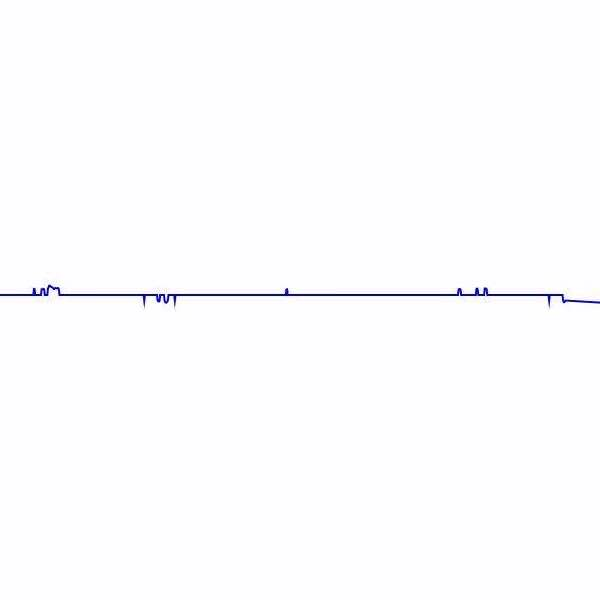
\includegraphics[height=4cm]{sound1.jpeg}}%
  \hspace{4em}%
  \subcaptionbox{某次点击的声音波形}
      {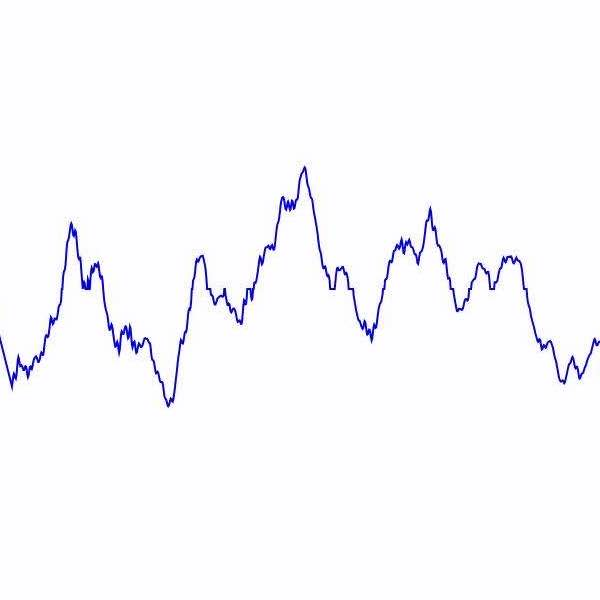
\includegraphics[height=4cm]{sound0.jpeg}}
  \caption{有无点击的声音波形对比}
  \label{fig:sound-comp}
\end{figure}

可以看出,正常无点击时波形较平,环境噪音只有很小的干扰。但是发生点击时,波峰波谷十分明显。因此,可以通过计算在一段时间窗口内数据流中超过某个阈值的数据个数判断是否有点击发生。

每帧的数据为两个字节,根据我们的经验,周围声音的响度一般低于1000,正常点击的峰值会大于3000,最终我们将3000设为阈值。此外,为了减少误识别,我们还将两次点击的最小间隔设置成50ms。通过预实验,发现除了环境中有十分类似点击的其他声音外,正常情况下该阈值的设定能够准确地识别用户的点击。

\section{深度数据的处理}
深度数据是支持我们此项工作的核心,手机前置深度数据使得任意桌面上文本输入的从全新的角度大大增加了可能性。

我们获取的数据为30Hz,维度为640*480的深度图像,其中每个像素点的数值代表手机离该点的距离。图~\ref{fig:depth1}中展示了用户端坐在手机前的原始的深度图像,在该图中,我们能够较为明显地分辨出用户上身的轮廓,包括双手、头部等以及环境中其他物体。其中,距离近的物体在图中黑色更显著,例如双手。

通过距离信息,我们可以去除图像后景无关的信息,只保留用户手部。考虑到用户距离手机的位置,我们只保留15-40cm范围的图像信息,据此对原图加以处理后得到的图像为~\ref{fig:depth2},可以看到,用户的手部被十分完好的保存了下来,其他的部分则被过滤了。
\begin{figure}[h]
  \centering%
  \subcaptionbox{原始深度图像\label{fig:depth1}} %标题的长度,超过则会换行,如下一个小图。
    {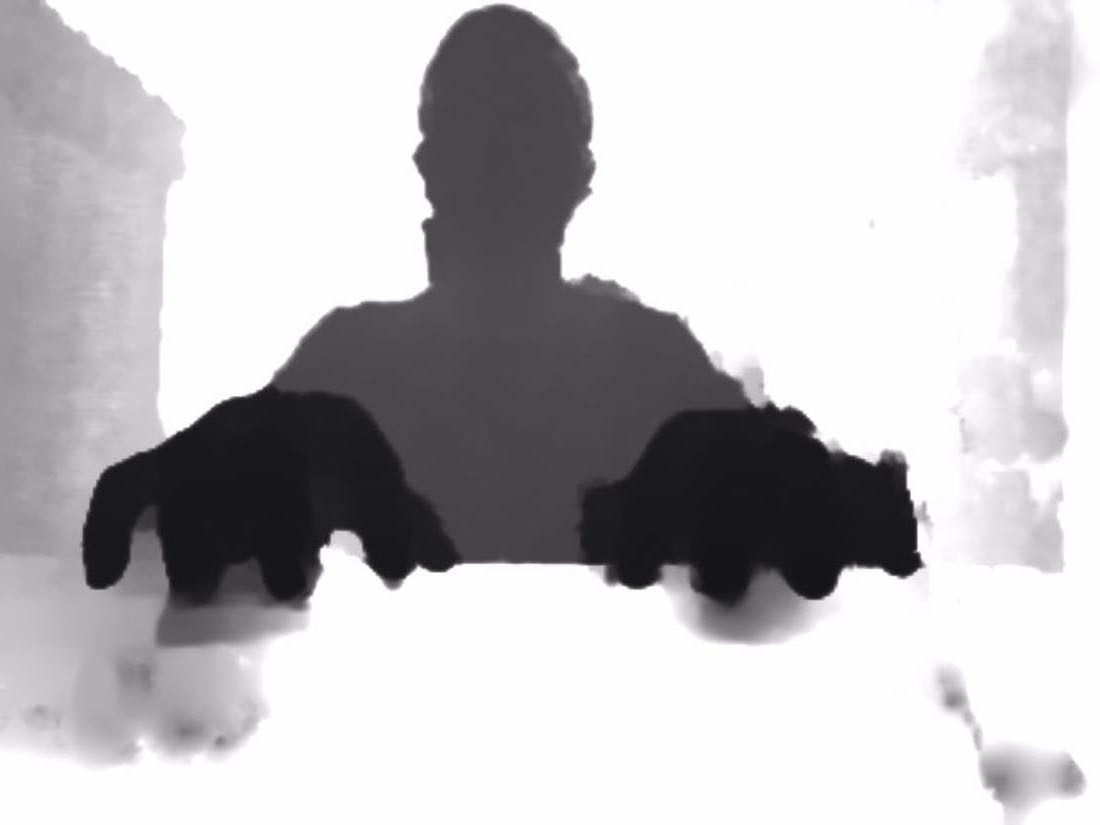
\includegraphics[height=4cm]{depth0.jpeg}}%
  \hspace{4em}%
  \subcaptionbox{处理后的深度图\label{fig:depth2}}
      {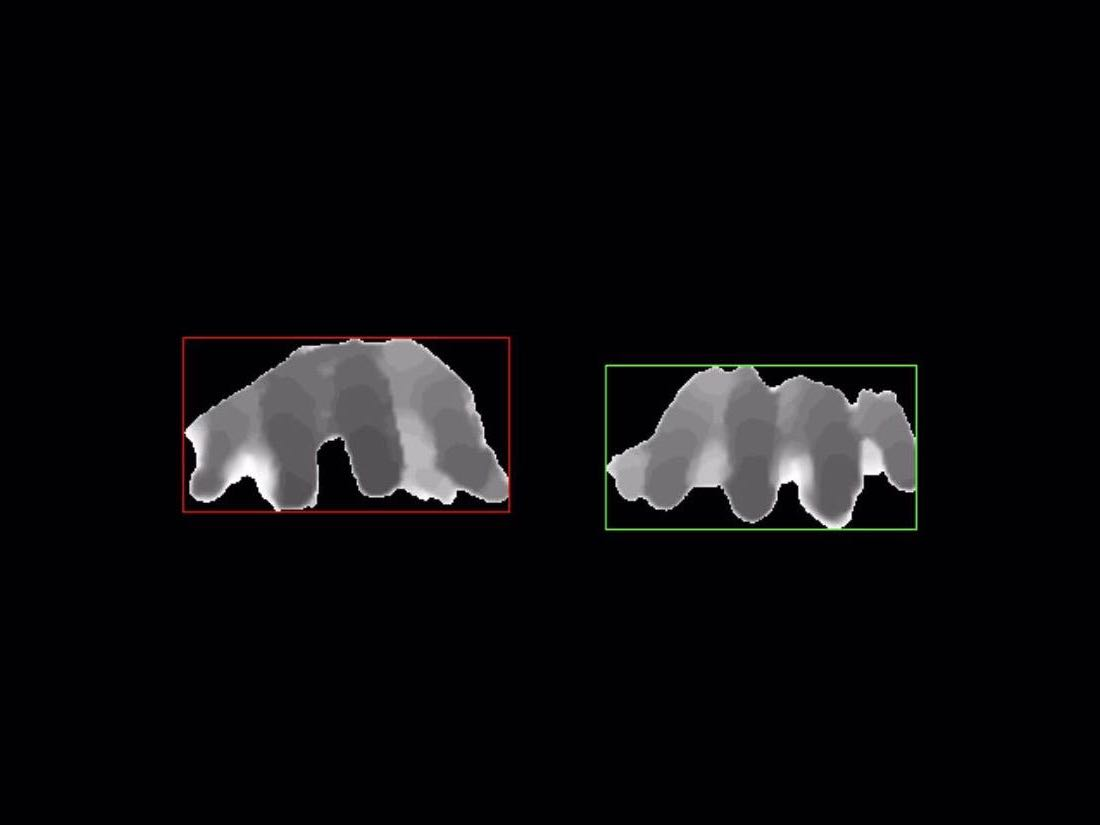
\includegraphics[height=4cm]{depth1.jpeg}}
  \caption{处理前后的深度图像}
  \label{fig:depth-image}
\end{figure}

获取处理后的深度图像后,我们首先识别出图中所有的轮廓,其中面积最大的两个即为用户的手部。当用户手部从悬浮状态发生点击时,点击的手指会位于深度图像最低点。基于这一事实,当通过声音检测到点击时,我们首先寻找到手部轮廓和外接矩形的最低点。

在图中找到最低点后,接下来便是计算点击位置离手机的距离。根据我们的尝试,由于指缝等的干扰,直接在深度图中读取点击处的像素深度可能会出现一定的误差,因此我们在该位置的领域进行洪范后计算距离的平均值。如果出现识别出多个切点的情况,我们选择距离最近的一个。

此外,基于深度图像的信息,我们不仅可以区分双手,同时还能够监测手部的运动状态,提供了左手左移和右手右移的手势。
%ring queue
%手指识别

\section{三维坐标的计算}
前面部分已经提到了如何计算点击和手机的距离,本节将介绍如何进一步计算该点击在物理世界中的三维坐标。

相机的成像,简言之,指的是将现实世界三维空间中的点映射成为图片中二维空间中的点这一过程,即将世界坐标系中的三维坐标转化为像素坐标系的二维坐标。其原理可以用式~(\ref{imageform})表示。
% 为了获得该过程的映射关系,一般需要引入以下几个坐标系:
% \begin{itemize}
%     \item \textbf{世界坐标系:}指的是物体在三维世界中的位置,一般由相机指定,用$(U, V, W)$表示
%     \item \textbf{相机坐标系:}以相机的光心为坐标系原点,到成像平面的距离为焦距,可由世界坐标系旋转和平移得到,用$(X, Y, Z)$表示
%     \item \textbf{图像坐标系:}在成像平面上的二维坐标系,用$(x, y)$表示
%     \item \textbf{像素坐标系:}最终图片的像素坐标,也在成像平面上,由图像坐标系平移和缩放得到,用$(u, v)$表示
% \end{itemize}

\begin{equation}
    \label{imageform}
    \begin{aligned}
    \begin{bmatrix}
        u \\
        v \\
        1
    \end{bmatrix}
    &= \frac{1}{Z} \begin{bmatrix}
        f / s_x & 0 & o_x & 0\\
        0 & f / s_y & o_y & 0 \\
        0 & 0 & 1 & 0
      \end{bmatrix}
      \begin{bmatrix}
        R & t \\
        0^{T} & 1
      \end{bmatrix}
      \begin{bmatrix}
        U \\
        V \\
        W \\
        1
      \end{bmatrix} \\
    &= \frac{1}{Z} \begin{bmatrix}
        f / s_x & 0 & o_x & 0\\
        0 & f / s_y & o_y & 0 \\
        0 & 0 & 1 & 0
      \end{bmatrix}
      \begin{bmatrix}
        X \\
        Y \\
        Z \\
        1
      \end{bmatrix}
    \end{aligned}
\end{equation}

式~(\ref{imageform})中的$(X, Y, Z)$为我们要求的点击在物理世界中的坐标,而$(u, v)$则是我们前文获得的点击在深度图像中的位置。$f$,$s_x$,$s_y$,$o_x$,$o_y$,$R$,$t$都属于相机的参数,可通过对应接口获取。

在本工作中,我们已经得到了点击位置在世界坐标系中的深度坐标$Z$。此外,在我们的设备中,相机坐标系和世界坐标系只是将$X, Y$调换为$V, U$。因此,前述的公式可以化简为公式~(\ref{equ:world-coord})。这样,我们便得到了一次点击的全部三维信息。由于我们在使用时手机靠于墙壁,和桌面垂直,即$Y$方向垂直桌面,因此$Y$坐标基本为定值。后文中主要用到$X$和$Z$方向坐标,为了表述方便,仍然称之为横轴和纵轴。
\begin{equation}
  \begin{aligned}
  X &= \frac{(u - o_x)s_x}{f_x} \times Z \\
  Y &= \frac{(v - o_y)s_y}{f_y} \times Z
  \end{aligned}
  \label{equ:world-coord}
\end{equation}

\section{点击识别算法流程}
根据本章前面部分描述的声音信号和深度图像处理的内容,我们可以搭建出整个的点击识别算法框架,表述为伪代码如下。

算法首先通过声音识别点击,然后查看双手是否在合适的范围内,如果有手势则先处理手势,没有手势则计算点击坐标。
\begin{algorithm}[h]
  \caption{点击识别算法伪代码} %算法的名字
  \hspace*{0.02in} {\bf Input:} %算法的输入, \hspace*{0.02in}用来控制位置,同时利用 \\ 进行换行
  声音数据流、深度数据流\\
  \hspace*{0.02in} {\bf Output:} %算法的结果输出
  点击的世界坐标
  \begin{algorithmic}[1]
  % \State some description % \State 后写一般语句
  \If{Tap Detected}
    \If{Hands in Range}
      \If{Gestures Detected}
        \State Process gestures
      \Else
        \State Find the tangent point of hand contour and its bounding box
        \State Calculate the tap coordinate in world coordinate system
        \State \Return tap coordinate
      \EndIf
    \Else 
      \State Marked as invalid tap 
      \State \Return
    \EndIf
  \EndIf
  % \For{condition} % For 语句,需要和EndFor对应
  %   \State ...
  %   \If{condition} % If 语句,需要和EndIf对应
  %     \State ...
  %   \Else
  %     \State ...
  %   \EndIf
  % \EndFor
  % \While{condition} % While语句,需要和EndWhile对应
  %   \State ...
  % \EndWhile
  % \State \Return result
  \end{algorithmic}
\end{algorithm}
% !TeX root = ../main.tex
\chapter{实验一:用户任意桌面点击行为规律}
\label{cha:exp1}
虽然相关文献已经表明用户能够将双手盲打的肌肉记忆迁移到不同的应用场景,例如大尺寸触摸屏、单手输入等等。然而,由于我们的交互界面并非触摸屏,而是一般的桌面,由于材质不同,用户输入时的触感也有一定差异。因此我们通过此实验进一步探究在普通桌面上用户双手输入的习惯和行为规律。


\section{被试}
在桌面上十指输入的实验中,我们一共招募了X名被试(男性X人,女性X人),平均年龄为X岁(标准差=X)。所有人都具有在物理键盘上熟练打字的使用习惯。此外,在正式实验开始前,我们首先使用Wobbrock编写的TextTest软件\cite{texttest}\cite{wobbrock2006analyzing}测试了他们在实体键盘上的打字速度和准确度。经过测试,被试们的输入速度为X单词每分钟,无纠正情况的错误率为X\%。每位被试获得50元作为实验报酬。

\section{实验装置和实验平台}
\begin{figure}[h] % use float package if you want it here
    \centering
    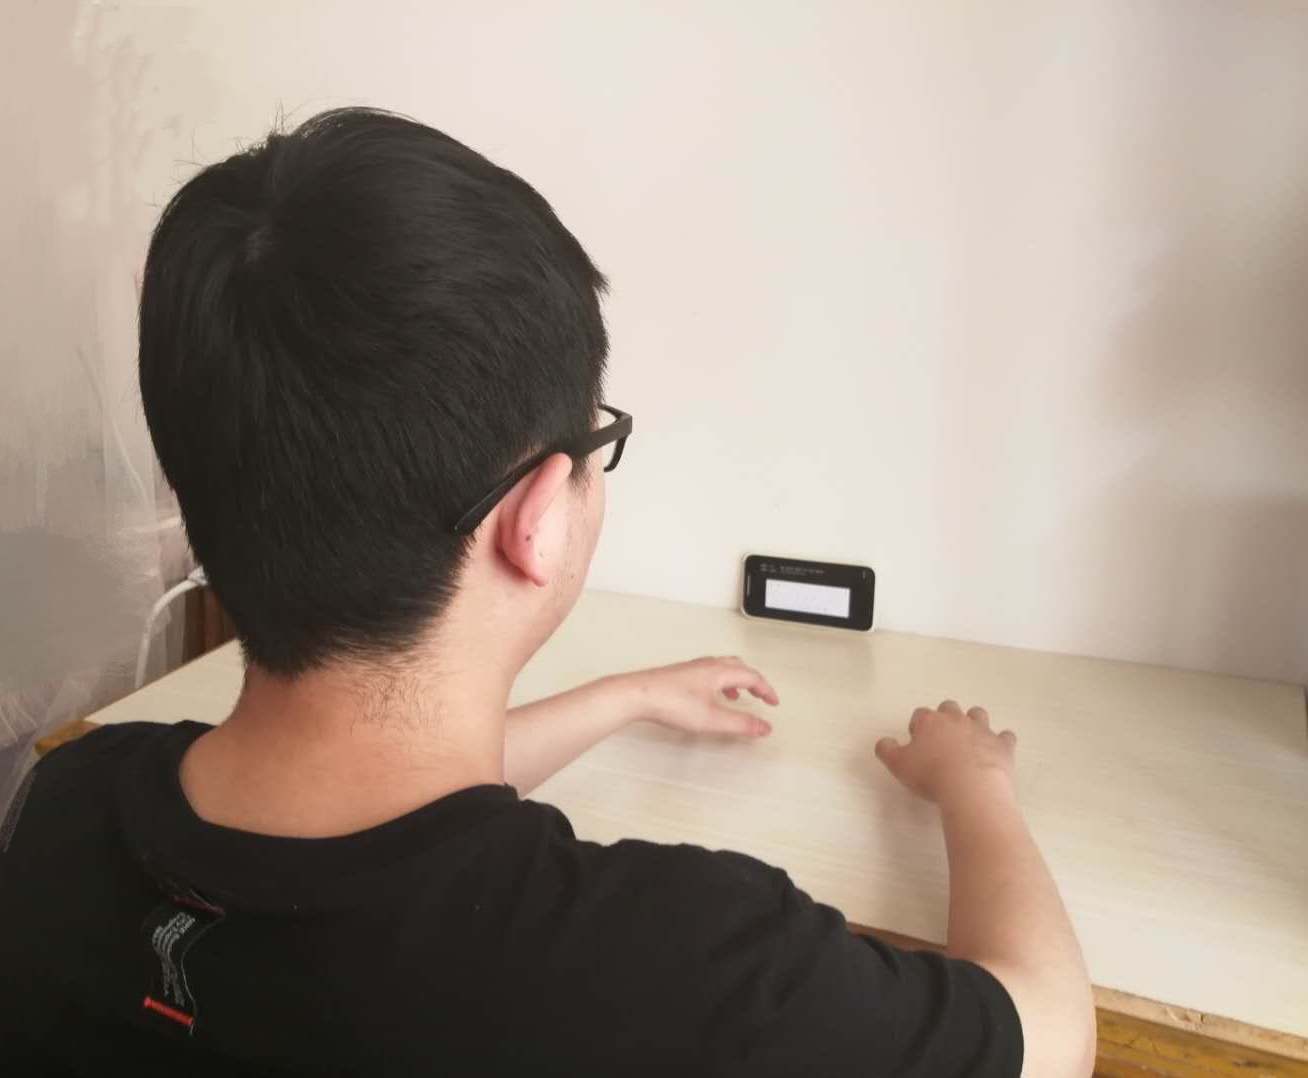
\includegraphics[height=6cm]{exp.jpeg}
    \caption{用户在桌面上输入的场景}
    \label{fig:exp}
\end{figure}
我们使用Swift和Objective-C在iPhone 11上开发了APP作为实验平台,XCode为开发环境。其中第~\ref{cha:sensing}~章已经对于手机如何获取并处理传感信息做了具体介绍,我们程序记录下了每次点击的坐标位置和相应时间戳。手机不仅用来接收传感信号,同时也向用户展示了实验平台。手机的屏幕尺寸为6.1英寸。在使用时,用户的双手距离手机约15-30厘米。为了充分利用手机的视场角,用户两手中心和手机的前置摄像头基本处于同一竖直线上。这样摄像头能够较为完整捕捉到手部的运动信息。图~\ref{fig:exp}~展示了用户进行实验时的状态。为了避免外界声音的干扰,实验在较为安静的室内空间进行。

图~\ref{fig:platform0}~展示了实验时手机上的界面。界面上显示了当前的实验进度以及用户要输入的目标句子。另外,为了防止用户遗忘物理键盘布局,我们在界面下方放置了一个标准的QWERTY键盘作为参考。

\begin{figure}[h] % use float package if you want it here
    \centering
    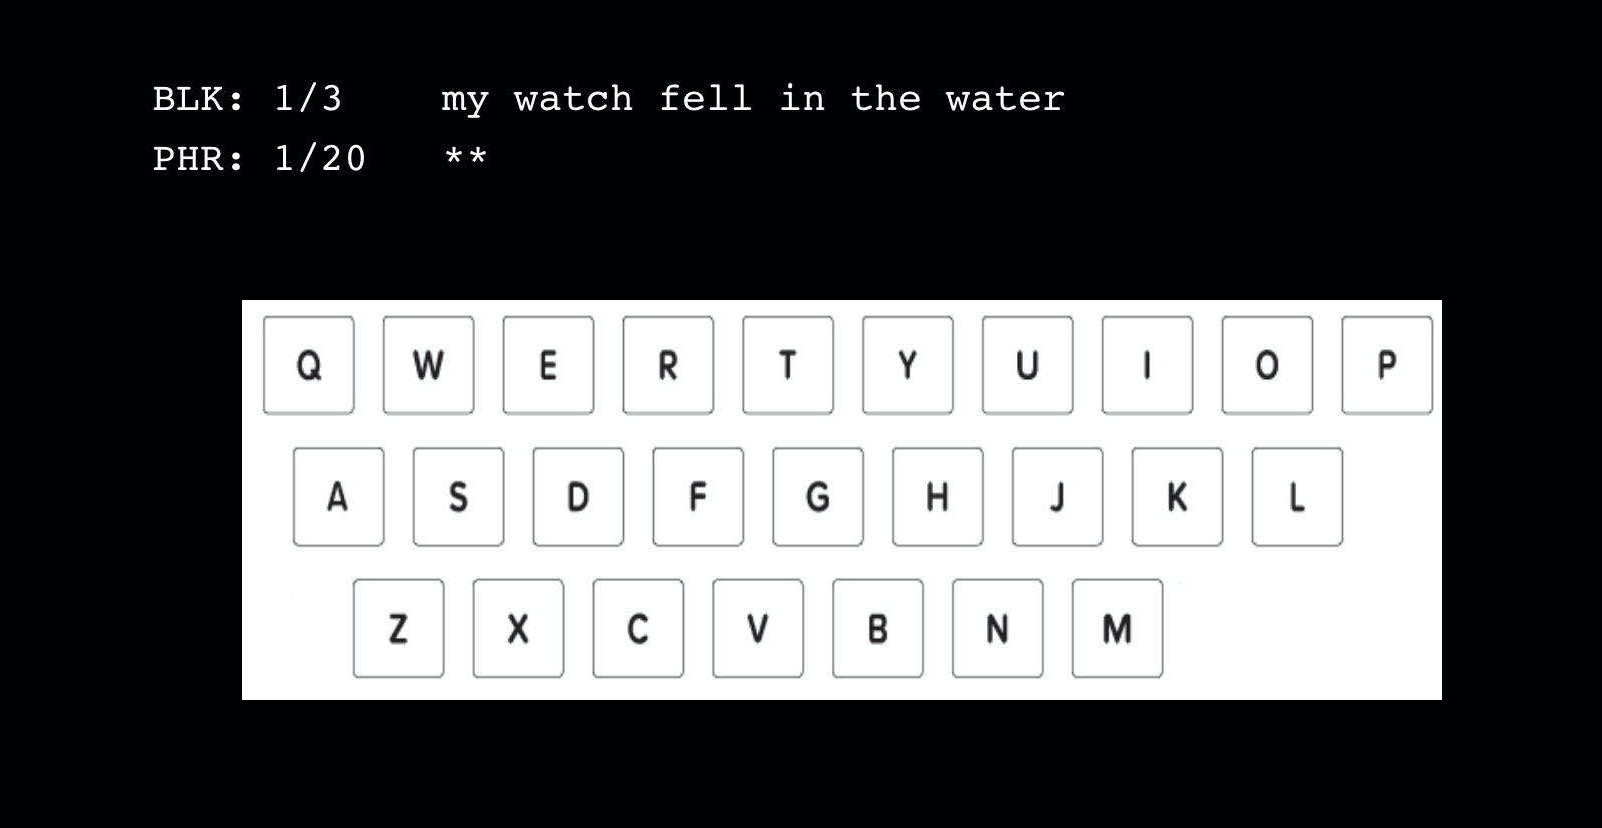
\includegraphics[height=5cm]{platform0.jpeg}
    \caption{iPhone11上实验平台界面}
    \label{fig:platform0}
\end{figure}

和前人工作类似\cite{flatglass2011findlater}\cite{2017blindtype},在打字的过程中,如图~\ref{fig:platform0}~所示,我们提供星号作为视觉反馈。这是为了尽可能减小不同输入纠错算法对用户本身的输入行为造成影响。另外,基于第~\ref{cha:sensing}~章的点击识别算法,每次识别到用户的点击,星号的数目会相应增加一个。


\section{实验设计及流程}
每位用户一共需要输入60句话,分为4部分,我们称为输入块。每个输入块一共有15句话,其中有13句是从Mackenzie提出的短语库\cite{mackenzie2003phrase}中随机选择的,另外两句均是相同的全字母句“The quick brown fox jumps over the lazy dog”和“The five boxing wizards jump quickly”,保证了每个用户都能够输入字母表中所有字母。

用户坐在手机前进行整个实验流程。在实验开始前,我们会简要介绍实验的目的并且指示用户尽可能快而准确地输入。用户将有3分钟的时间用于熟练实验平台。每当用户输入完一句话后,右手进行右移进入下一个句子。为了防止手部疲劳,每输入完一句话用户可以将手放在桌面上休息,每输入完一个输入块用户会需要强制休息2分钟。此外,当用户察觉到自己输入错误时,可以左手左划清空本句的数据并重新输入。实验结束后,我们会搜集用户的基本信息,并针对输入体验、速度、使用习惯等问题以及相关建议对用户进行一个简要的访谈。

\section{实验结果}
从XX名用户的数据中,我们一共收集了XX个落点。为了减小偶然误差的影响,对于每个按键,我们移除了各方向超过3倍标准差的落点,一共有XX个,占所有落点XX的比例。

\subsection{输入速度}
我们输入速度的计算使用MacKenzie提出的公式\cite{speedcalc},单位是WPM,即单词每分钟。

\begin{equation}
    \label{calcspeed}
    WPM = \frac{|L|-1}{T} \times 60 \times \frac{1}{5}
\end{equation}

其中,$|L|$是输入的某段文本的长度,在我们的计算中即从一句话第一个字符到最后一个字符所有字符数,$T$是输入这句话所用的总时间,单位为秒。

输入的平均速度为43(SD = XX)WPM,速度范围为XX WPM到XX WPM,该速度要慢于在物理键盘上的速度。从图~\ref{fig:speed0}~中可以看出,输入速度随着输入块单调递增,在最后一个输入块能够超过45WPM。平均速度快于同样有星号反馈情况下在触摸屏上十指盲打\%\cite{flatglass2011findlater},慢于物理键盘上的平均输入速度。速度的趋势说明用户能够逐渐适应并熟练掌握在桌面上输入的方式。F检验证明输入块对于输入速度有显著的影响(F=XX, p=XX)。
\begin{figure}[h] % use float package if you want it here
    \centering
    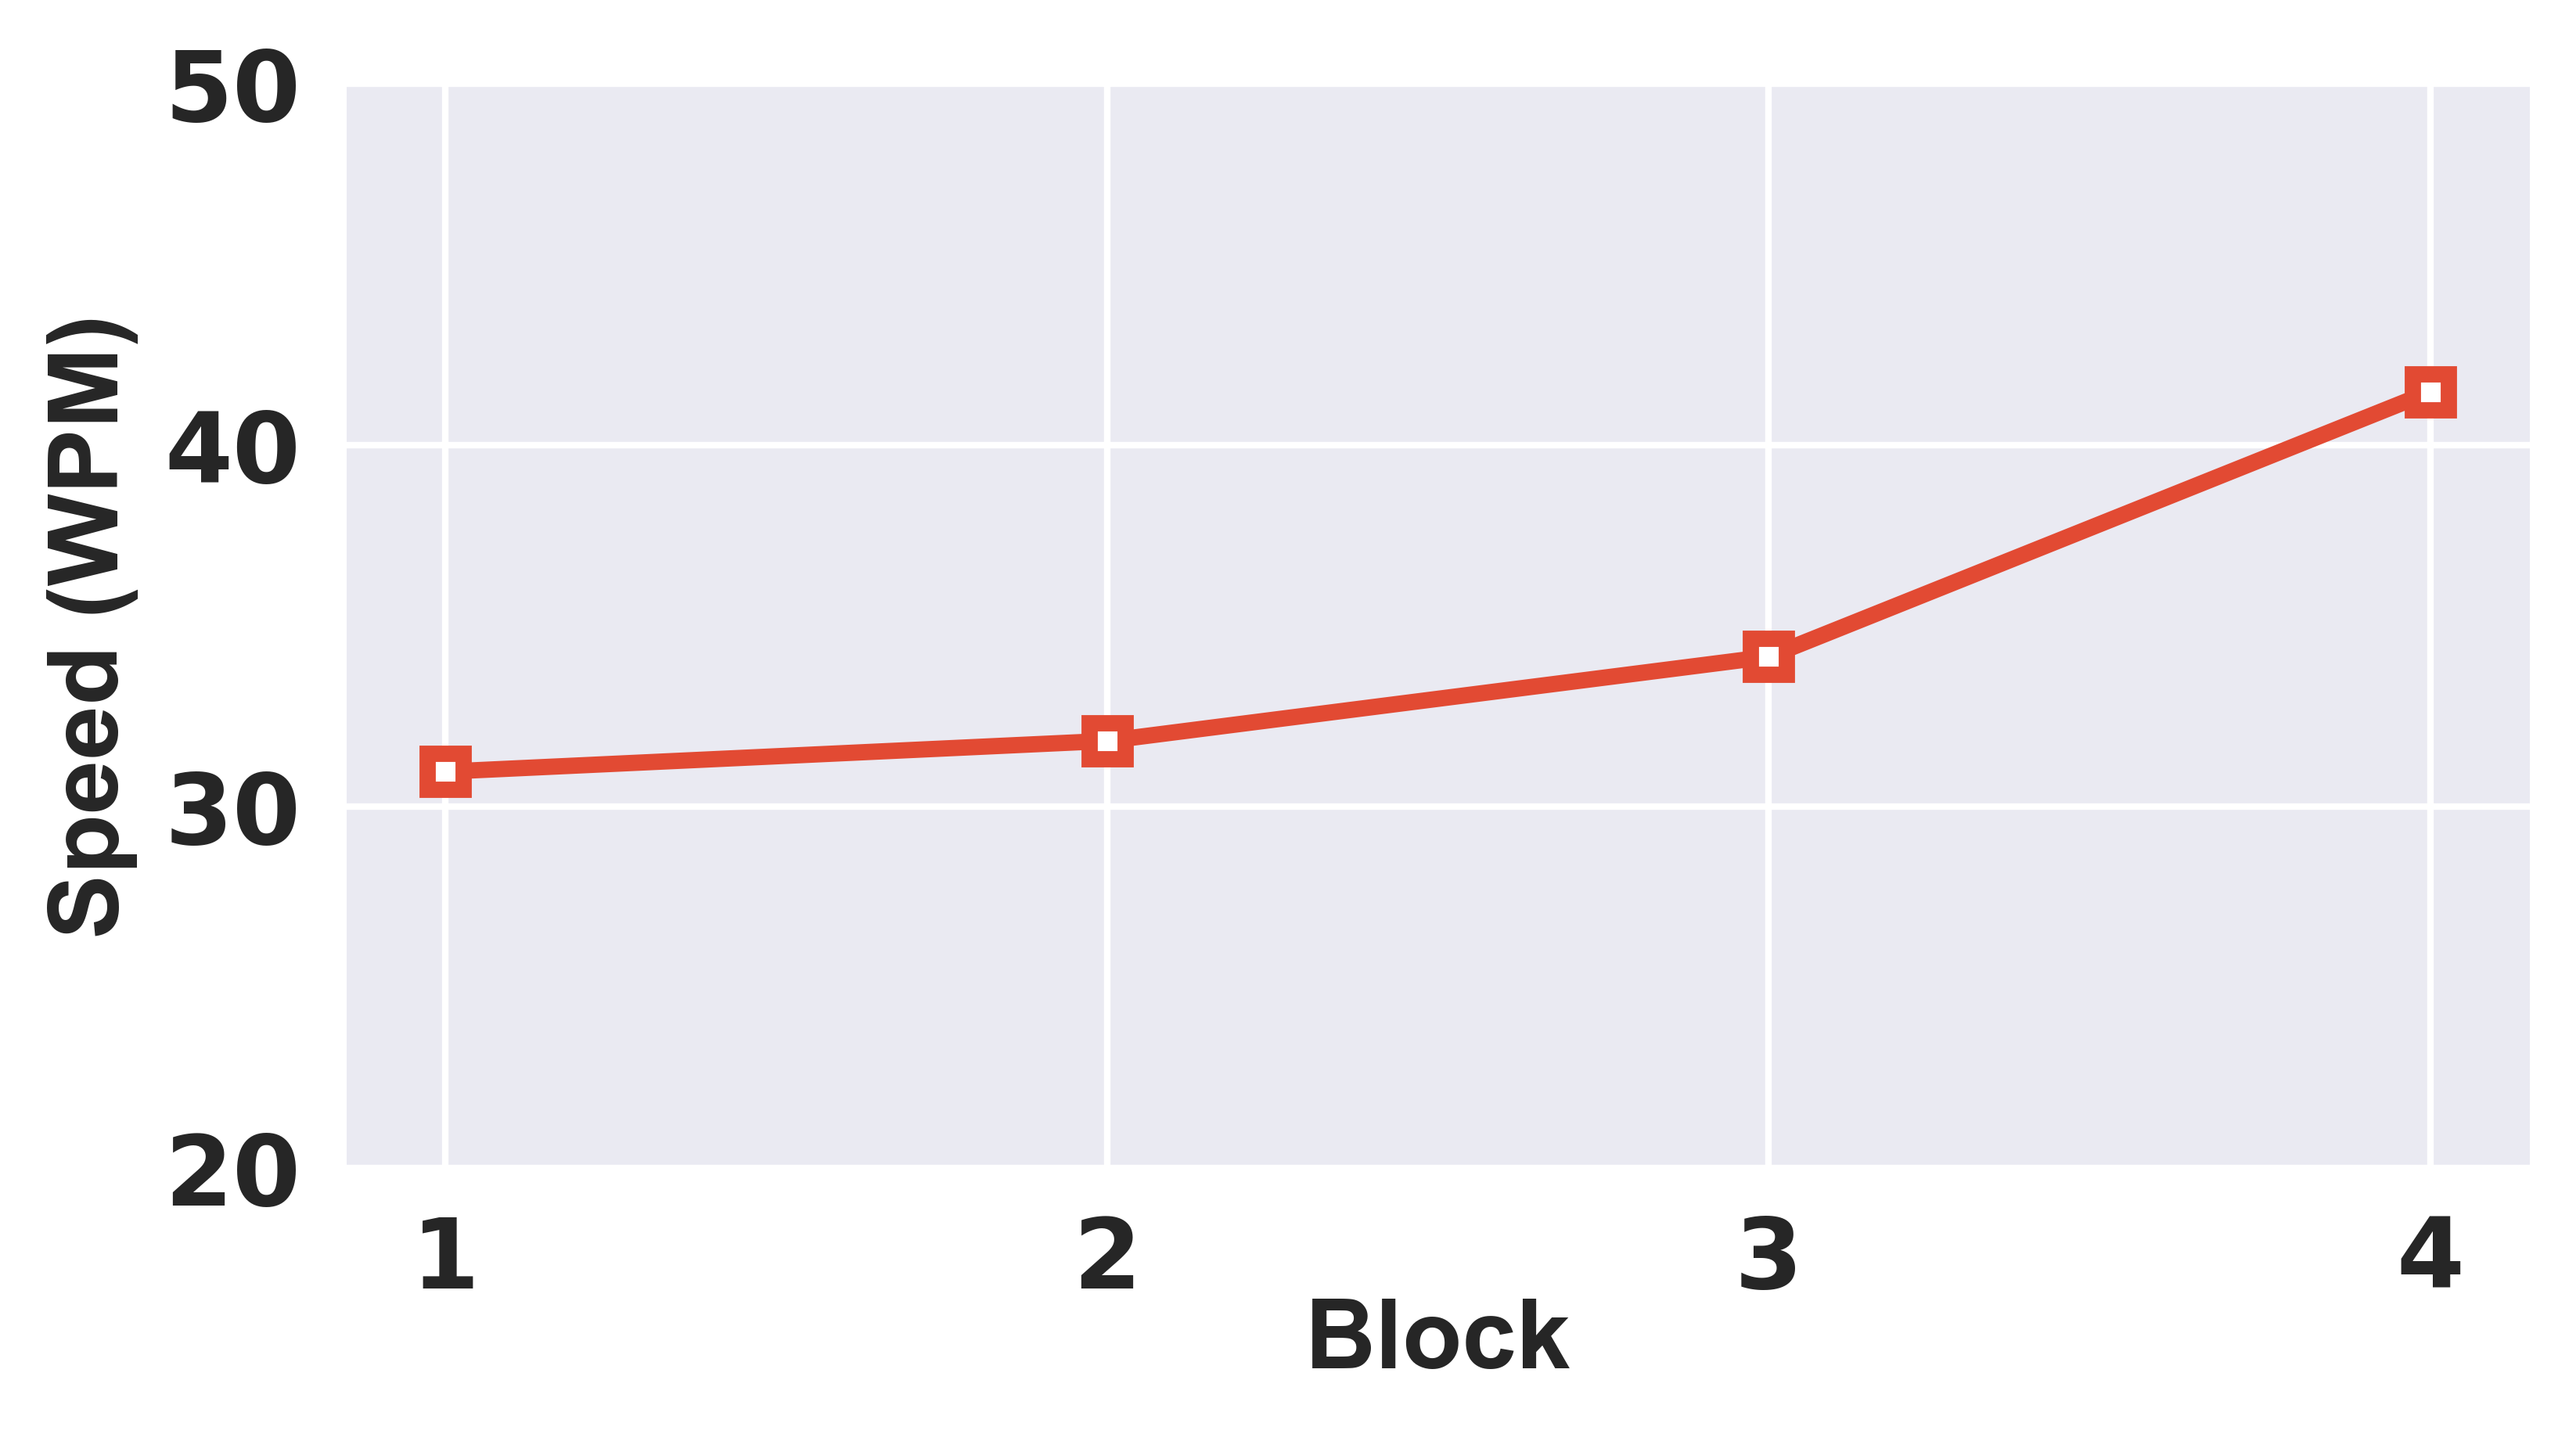
\includegraphics[height=6cm]{speed0.png}
    \caption{实验时每个输入块的平均输入速度}
    \label{fig:speed0}
\end{figure}

\subsection{落点分布}
考虑到不同用户落点分布的绝对位置有一定偏差,我们将所有人F键和J键的中心点平移到了同一位置进行进一步分析\cite{flatglass2011findlater}\cite{palmboard2020}\cite{2018shitoast}。图~\ref{fig:points}~展示了所有用户落点集中后的分布图,可以看出每个按键呈聚集的趋势,但是相邻的按键,尤其是同一行的按键有一定的重合。

\begin{figure}[h] % use float package if you want it here
    \centering
    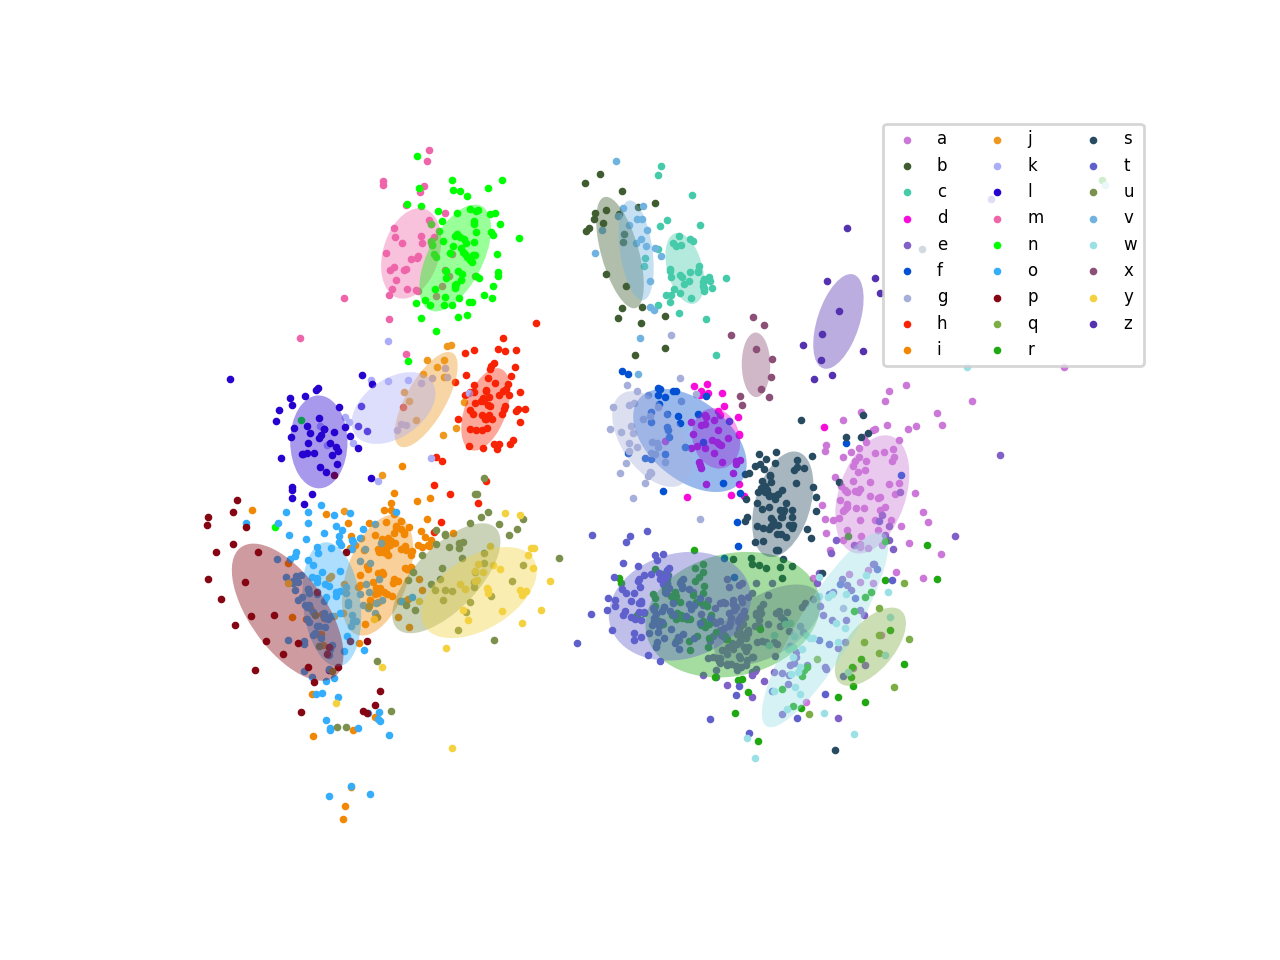
\includegraphics[width=13cm]{touchpoints.png}
    \caption{所有用户的落点分布图,使用颜色区分按键}
    \label{fig:points}
\end{figure}

表~\ref{tab:sd}~展示了字母键和空格键在单人情况下和合并情况下的在横轴和纵轴的标准差。其中平均而言,横轴标准差总是大于纵轴,说明被试相对而言更容易控制纵向的点击,因为横向同一行的按键更多,可能更难控制。然而,底部行(z,x按键所在行)在纵轴上的标准差更大,和文献中结果类似\cite{flatglass2011findlater}。此外,合并后的标准差要大于每个人单独计算的值,说明不同用户的输入控制能力存在一定差异,可能与平时键盘的使用习惯以及手指大小等因素有关。另外,无论是在单人还是所有人的情况下,空格键在两个方向上的标准差均远大于普通字母键,说明在无键盘的情况下,用户心理键盘模型中,空格键仍然和物理键盘上一样占据较大区域。

\begin{table}[htb]
    \centering
    \begin{minipage}[t]{0.7\linewidth} % 如果想在表格中使用脚注,minipage是个不错的办法
    \caption[实验一标准差]{单个人和所有人落点合并在一起的字母键和空格键在X和Y方向的标准差的平均值,括号中为不同人的标准差,其中第二行无标准差}
    \label{tab:sd}
      \centering
      \begin{tabularx}{0.7\linewidth}{c c c}
        \toprule[1.5pt]
        坐标轴 & X & Y\\\midrule[1pt]
        字母键(单人) & 1.1(1.1)& 1.1(1.1)\\
        空格键(单人) & &\\
        字母键(所有人) & & \\
        字母键(所有人) & &\\
        \bottomrule[1.5pt]
      \end{tabularx}
    \end{minipage}
  \end{table}

\subsection{键盘拟合}
使用BlindType\cite{2017blindtype}提出的公式~(\ref{equ:fitkeyboard})对用户点击进行键盘拟合。
\begin{equation}
  \label{equ:fitkeyboard}
  \begin{aligned}
  \textbf{x} &= s_{x} \times \textbf{X} + o_{x} \\
  \textbf{y} &= s_{y} \times \textbf{Y} + o_{y}
  \end{aligned}
\end{equation}

其中$\textbf{x}$和$\textbf{y}$为用户所有点击横纵坐标分别构成的向量,$\textbf{X}$和$\textbf{Y}$为$\textbf{x}$和$\textbf{y}$对应点击的按键在标准物理键盘上的横纵坐标。在两个方向分别进行线性回归,因此$s_{x}$和$s_{y}$表示拟合出的按键在两个方向上的长度,$o_{x}$和$o_{y}$为所拟合出键盘的偏移。表~\ref{tab:fitkeyboard}~中列出了拟合的全键盘按键大小及偏移。可以看到,因为可供用户输入的区域较大,拟合出的按键的尺寸也远大于物理键盘,并且纵轴长于横轴。图~\ref{fig:fitkeyboard}~展示了落点坐标轴的位置和方向,原点处是前置摄像头。根据拟合出的键盘偏移,图中展示了拟合后的键盘大致位置,和用户进行实验时双手放置位置一致。在两个方向上的$R^{2}$都超过了0.85,说明键盘拟合效果较好。

\begin{figure}[h] % use float package if you want it here
  \centering
  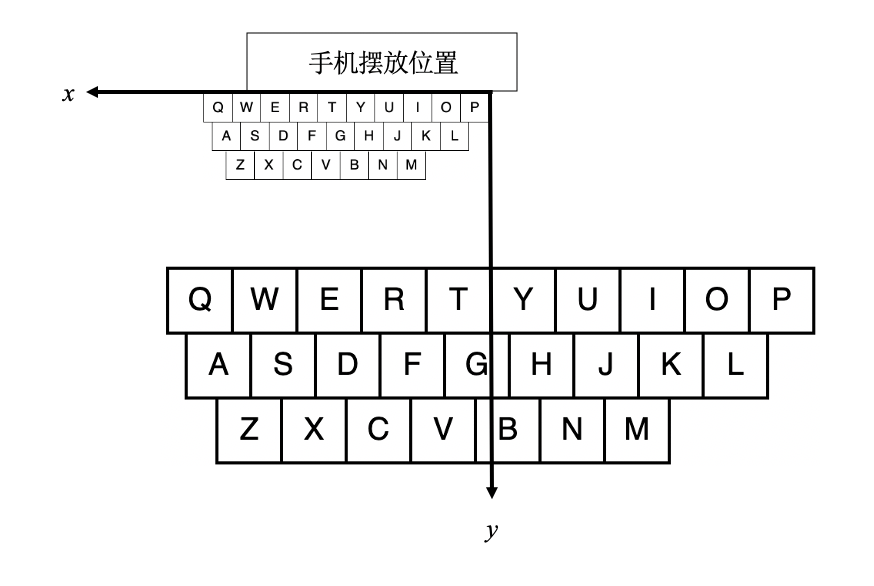
\includegraphics[width=10cm]{fit-keyboard.png}
  \caption{用户位置处的俯视图,较小键盘为拟合前的键盘位置,较大键盘显示了拟合后的位置和大小,实际比例可能有一定误差}
  \label{fig:fitkeyboard}
\end{figure}

\begin{table}[htb]
  \centering
  \begin{minipage}[t]{0.55\linewidth} % 如果想在表格中使用脚注,minipage是个不错的办法
  \caption[拟合出的键盘参数]{拟合出的键盘大小和偏移,括号中为标准差}
  \label{tab:fitkeyboard}
    \centering
    \begin{tabularx}{\linewidth}{cccc}
      \toprule[1.5pt]
      %  & \multicolumn{2}{c}{总体}&\multicolumn{2}{c}{左手} &  \multicolumn{2}{c}{右手} \\\midrule[1pt]
      & 按键大小(cm) & 键盘偏移(cm) & $R^{2}$ \\\midrule[1pt]
      X & 2.67 (0.24) & -13.17 (1.80) & 0.96 \\
      Y & 3.35 (0.38) & 20.24 (1.15) & 0.85\\
      \bottomrule[1.5pt]
    \end{tabularx}
  \end{minipage}
\end{table}

%spread of size
%两手之间的间距

\subsection{键盘落点分布}
图~\ref{fig:keyboard-curve}~展示了所有被试落点合并后的按键中心位置。从按键中心的分布情况可以看出,26个字母的相对位置仍然符合QWERTY布局。但是,不同于标准的物理键盘,落点分布呈现一定的弧形,和在触摸屏上十指盲打结果类似\cite{flatglass2011findlater}\cite{2018shitoast}。使用贝塞尔曲线分别拟合左右手每一行的按键中心如图\ref{fig:keyboard-curve}。

我们计算了最左到最右,最上到最下中心点的距离平均值,分别为22.8cm和7.97cm,可见落点分布范围较大,与拟合出的按键较大结果相一致。左右两只手的中间有一定间隔,说明用户在桌面上进行十指盲打时倾向于将两手分开并保持一定的距离,和在触摸屏上类似\cite{flatglass2011findlater}。
\begin{figure}[ht]
  \centering
  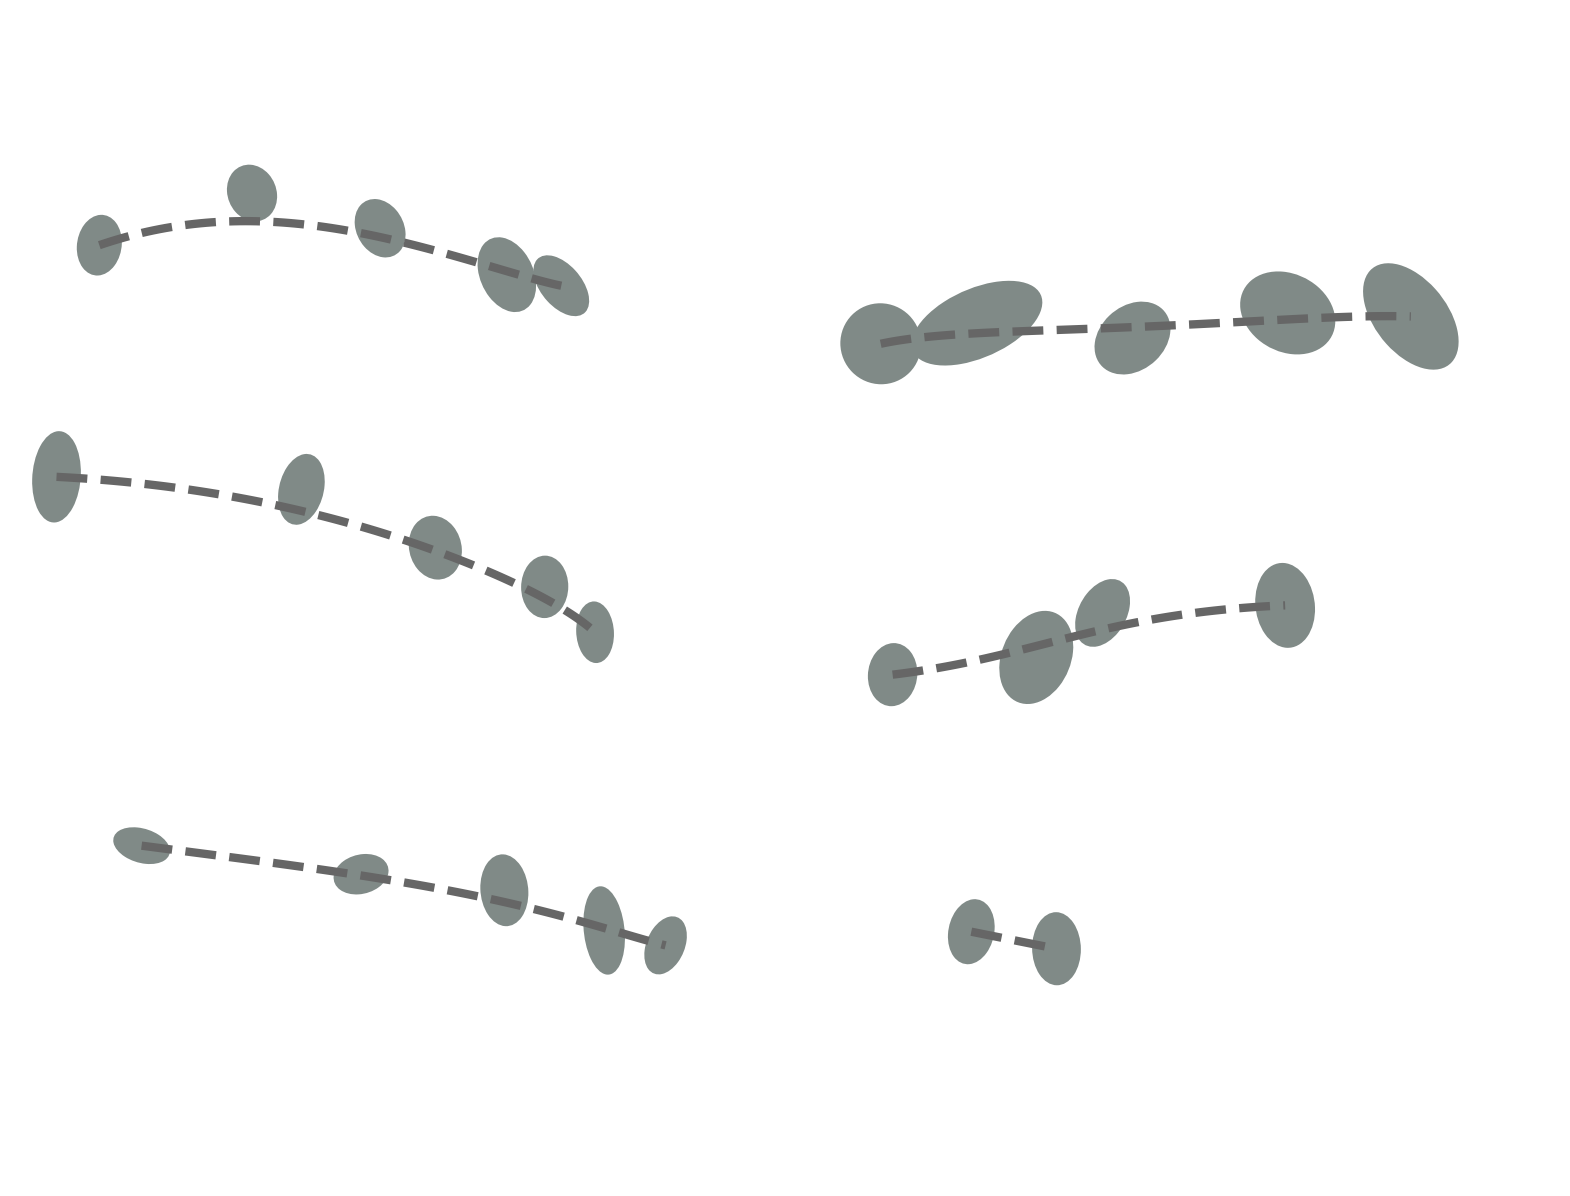
\includegraphics[height=6cm]{curve.png}
  \caption{使用贝塞尔曲线拟合的按键中心点,椭圆为一标准差}
  \label{fig:keyboard-curve}
\end{figure}

\subsection{输入行为}
在一般的触摸屏上例如iPad上十指输入时,因为误触的问题,用户在不输入时将双手放下休息。即使在没有误触时,因为心理因素,有的用户仍然习惯于不放下手\cite{palmboard2020}。在我们的实验中,我们允许并鼓励用户在输入完一个句子后将手放在桌面上休息。经过观察和访谈,我们发现用户愿意将双手放于桌面,并且用户称此行为能够减轻疲劳。

\section{本章总结}
本章通过用户实验,采集了用户在桌面上进行双手盲打的输入数据。我们分析了输入速度、按键大小、落点分布、输入行为等一系列特征,并对比了前人在触摸屏上类似实验。相比而言,我们的输入区域更大,因此拟合的按键也更大,并且能够较好支持用户双手放下休息的行为。
% !TeX root = ../main.tex
\chapter{用户输入意图推理算法探究}
\label{cha:algorithm}
\section{方法设计}
在本章中,我们通过上个实验收集的用户在桌面上的点击数据,进行模型实验,试图探究能够预测用户输入单词的推理算法。

对于每一种算法,我们的输入为用户的点击位置信息,输出为该算法预测出的概率最高的五个可能的单词。然后将其与正确的单词进行比对,分别计算对应的概率第一高到概率第五高的单词级别准确率。我们使用的是美国国家语料库,其中收录了各种正式和非正式场景下超过了2000万个单词。从该语料库中我们挑选了出现频率最高的10,000个单词作为词库,用于计算单词出现的概率。我们保证用户输入的单词都出现在词库中。
% !TeX root = ../main.tex
\chapter{实验二:真实使用场景下的评测} %字符级别输入的部分
\label{cha:evaluation}
根据上一章的模拟结果,我们将半键盘的相对算法集成到了系统中,作为我们单词级别输入的模型。此外,我们还在系统中实现了字符级别输入。在本章中,我们介绍了整个系统的设计,并对单词级别输入、字符级别输入和混合模式输入三种使用场景做了用户评测。

\section{平台设计}
% 平台图以及如何进行切换
\subsection{单词级别}
在单词级别的输入中,用户和实验一相同,将双手放置于手机前,在不显示键盘的情况下,按照自己的肌肉记忆在桌面上进行十指输入。

用户在进行输入时,平台的算法会根据用户点击的位置预测出用户可能的目标单词。屏幕上会显示出现概率最高的五个单词,用户可以使用右手右滑切换目标单词,和物理键盘相似,用户通过点击空格键选择当前光标的指向单词。如果用户认为自己输入出现错误,用户可以将左手左滑删除正在输入的部分或者删除上一个输入的单词。

\subsection{字符级别}
较为直观的输入字符的方式为显示完整键盘布局,用户移动到目标字符后进行选择。然而,由于手机的屏幕相对较小,且用户输入时眼部离手机有一定距离,因此若将所有字符完整显示在屏幕上不仅瞄准相对困难,且容易造成视觉疲劳。考虑到在单词级别输入时用户使用滑动的方式进行选择,我们字符级别的输入仍然采用类似的交互思路。

总体上我们使用二级菜单的设计,如图~\ref{fig:design}。其中第一级菜单为九宫格键盘,包括了26个英文字母和3个其他字符;当用户选择第一级菜单的某个方格之后,会出现二级菜单,二级菜单显示了对应方格的字符供用户进行选择。在一二级菜单中,用户均可以使用右手右滑向右移动光标,左手左滑向左移动光标以及任意手上滑 到达目标位置。仍然类似于单词输入,用户在一二级菜单进行选择时,可以使用右手任意手指进行点击。使用左手手指点击则对应退回的操作,如果当前在二级菜单则退回到一级菜单,如果在一级菜单则删除一个字符。

我们的系统支持两种模式混合输入。用户通过点击离手机较远的位置(35cm之后)切换输入模式,我们实验一的数据表明,用户在正常输入时超过30cm的点击比例小于0.1\%,且最远为32cm。另外,用户能够很容易判断如何快速点击合适位置进行切换。

\begin{figure}[htbp] % use float package if you want it here
    \centering
    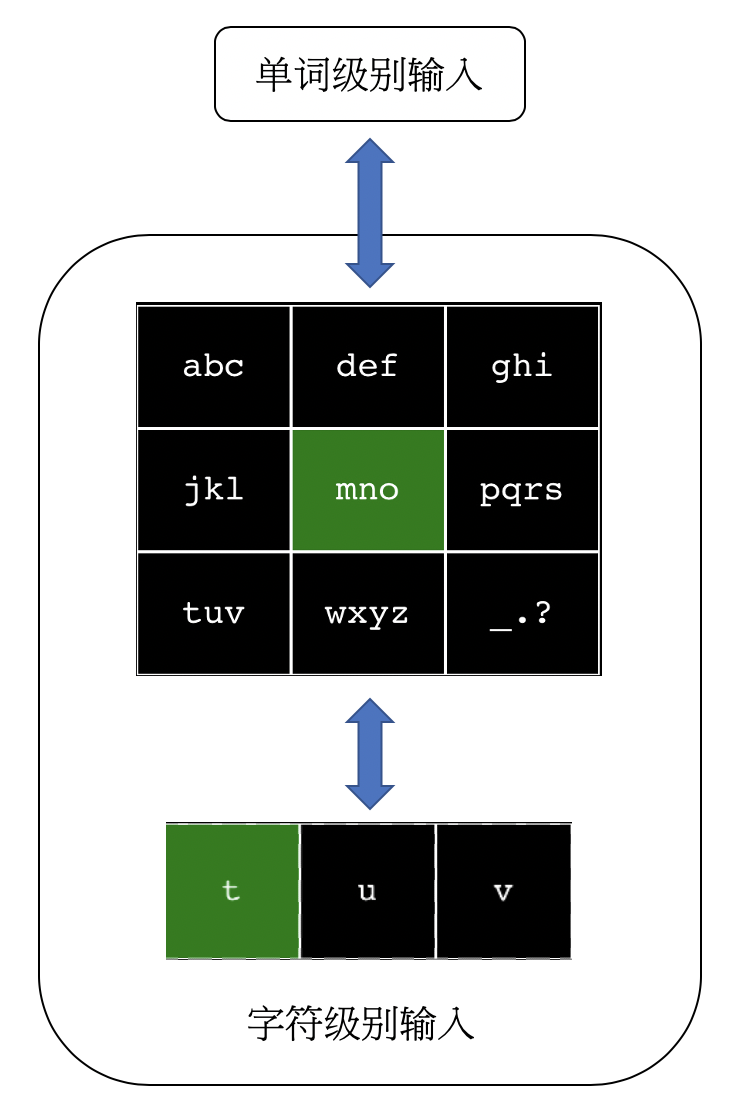
\includegraphics[height=11cm]{figures/design.png}
    \caption{平台设计结构图}
    \label{fig:design}
\end{figure}

\section{被试}
在评测实验中,我们招募了3名被试。被试们平均年龄为21.67岁(标准差=0.58),且均熟练使用实体键盘。我们仍使用了TextTest\cite{texttest}\cite{wobbrock2006analyzing}对他们物理键盘输入速度进行了测试,平均速度为59.3单词每分钟(标准差=8.86),无纠正错误率为0.06\%(标准差=0.04\%)。

\section{实验装置和实验平台}
本次实验的装置和实验一相同。实验平台同样类似,但是显示了当前的输入模式,在单词输入模式下多了一行单词供用户进行选择,在字符输入模式下显示一级或者二级菜单,见图~\ref{fig:platform1}。

\begin{figure}[h]
  \centering%
  \subcaptionbox{单词模式输入\label{fig:platform11}} %标题的长度,超过则会换行,如下一个小图。
    {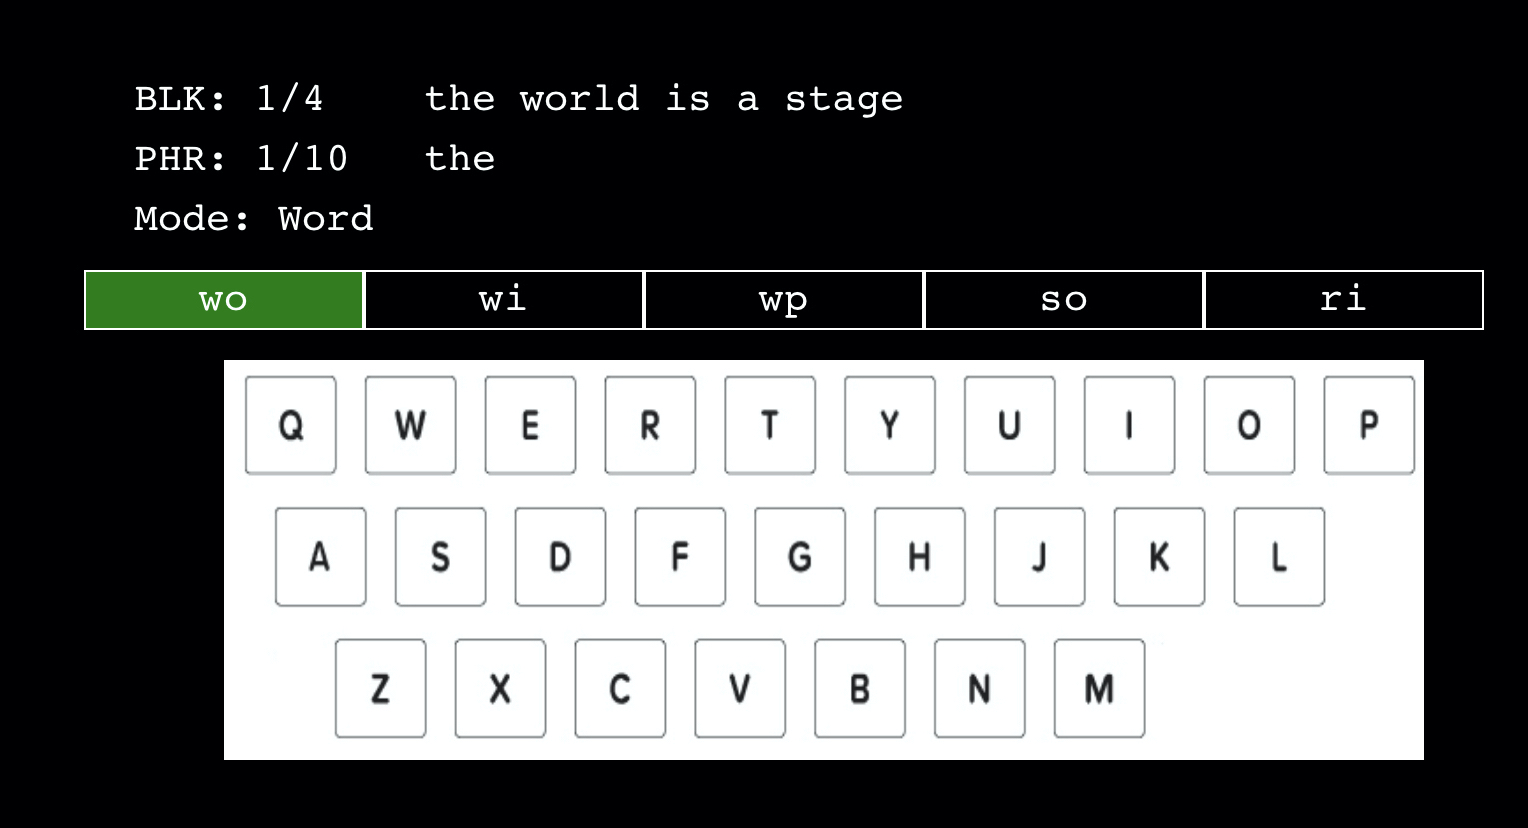
\includegraphics[height=5cm]{figures/platform11.jpg}}%
  \hspace{4em}%
  \subcaptionbox{字符模式输入\label{fig:platform12}}
      {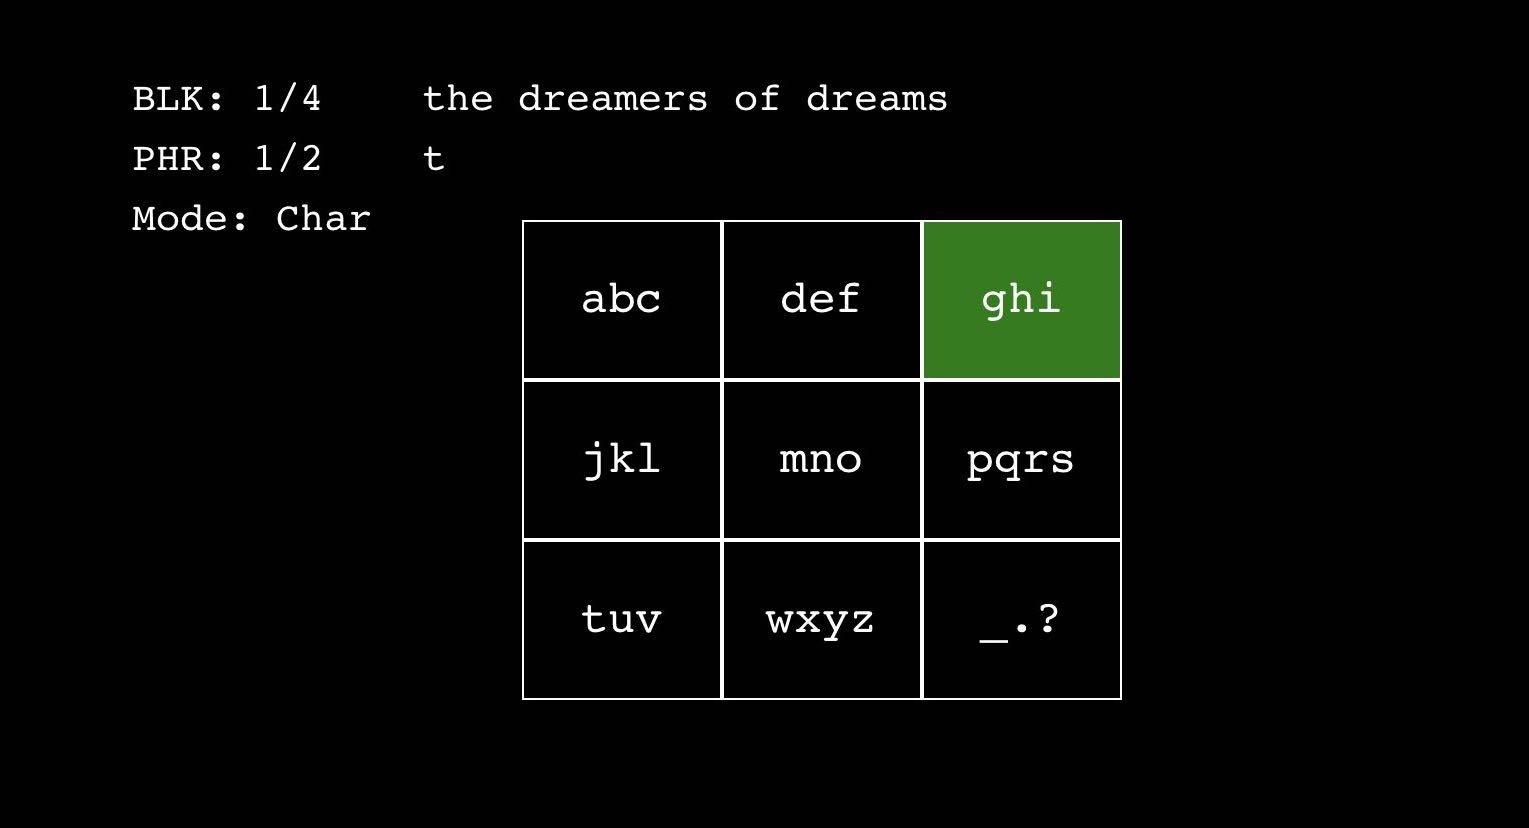
\includegraphics[height=5cm]{figures/platform12.jpg}}
  \hspace{4em}%
  \subcaptionbox{混合模式输入\label{fig:platform13}}
      {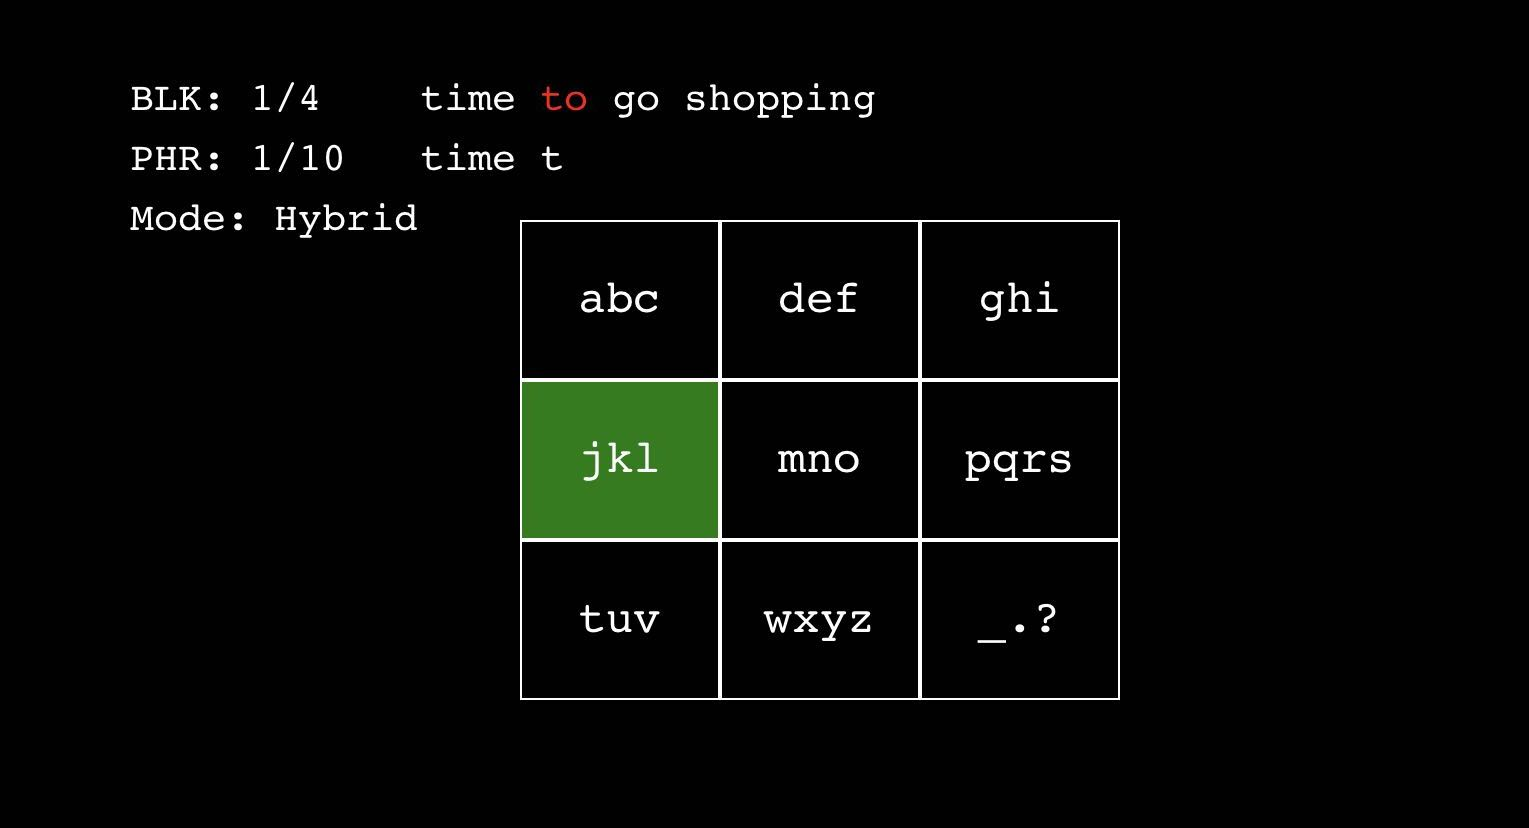
\includegraphics[height=5cm]{figures/platform13.jpg}}
  \caption{实验二平台截图}
  \label{fig:platform1}
\end{figure}


% \begin{figure}[h] % use float package if you want it here
%     \centering
%     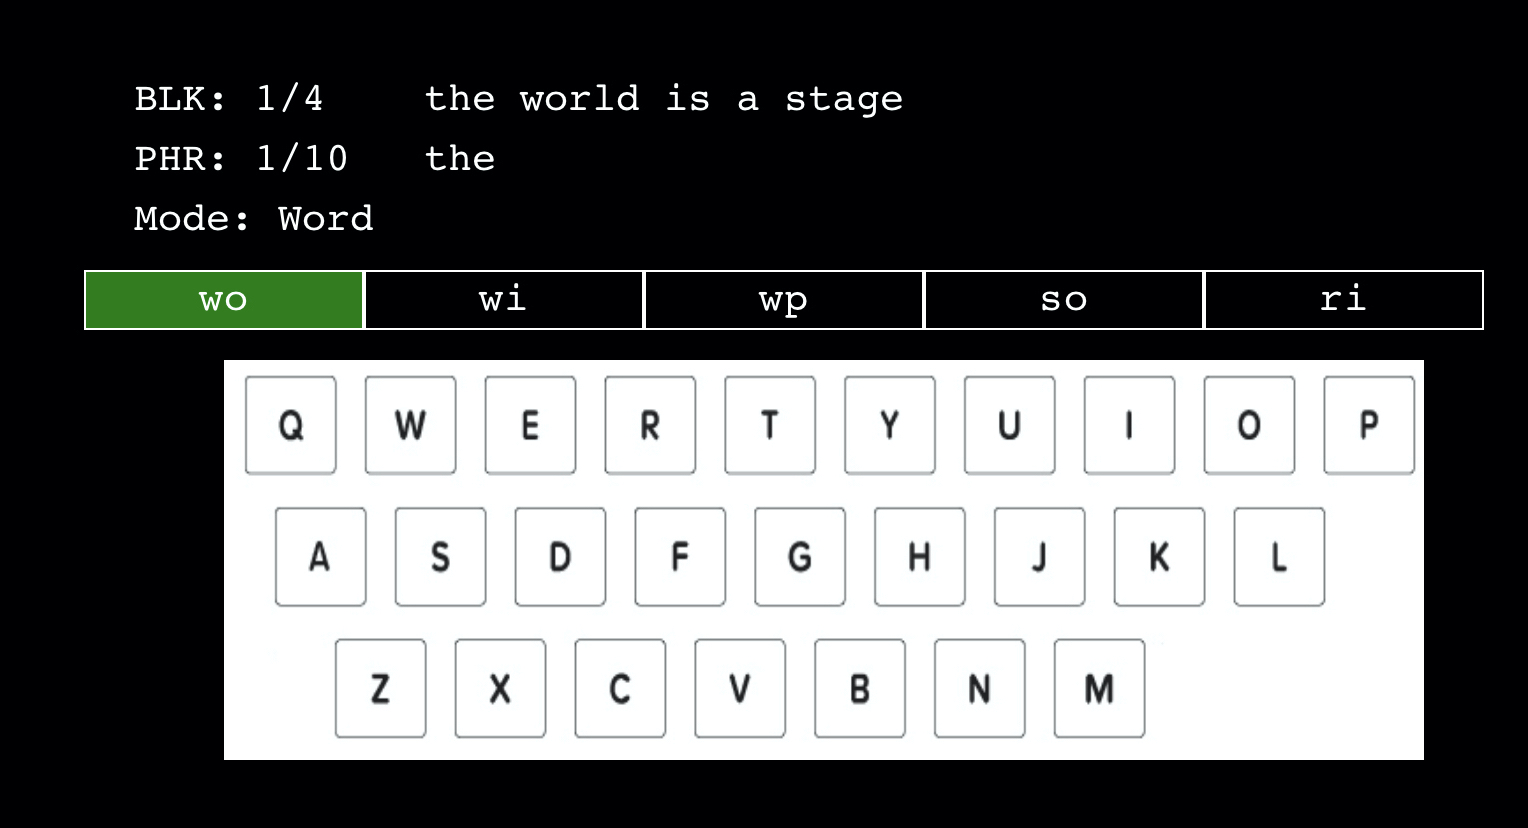
\includegraphics[height=5cm]{figures/platform11.jpg}
%     \caption{实验二平台截图}
%     \label{fig:platform1}
% \end{figure}

\section{实验设计和流程}
为了研究我们的平台在不同情况下的输入效率,评测实验分为三个模式,分别是单词模式、字符模式和单词字符混合模式。具体操作方式见本章平台设计部分。为了避免不同模式顺序对结果的影响,每位用户实验时先进行单词模式和字符模式输入,两者顺序随机,最后进行混合模式输入。屏幕上会标明当前的输入模式。在输入单词时,我们和第~\ref{cha:algorithm}~章一样,使用10,000个单词作为词库。

在单词模式和混合模式的输入中,用户需要完成4个输入块,每个输入块10句话,为Mackenzie句库随机选择而成\cite{mackenzie2003phrase}。其中混合模式下,每个句子中随机选择一个单词标红,用户必须通过逐个输入字符的方式拼出该单词,其余的部分则仍然输入整个单词。在字符模式下,用户同样完成4个输入块,每个输入块2句话,也为Mackenzie句库\cite{mackenzie2003phrase}打乱并挑选构成。为了使用户使用时更清晰方便,输入字符时使用'\_'表示空格。

在正式实验开始前,每位用户有10分钟的时间熟悉实验平台。在输入时,我们要求用户尽可能快而准确进行。每当用户输入完一句话后,用户可以点击任意按键跳到下一句。在输入块之间,用户需要强制休息2分钟。在完成一句后,用户也可以根据个人需求将手放在桌面上休息。实验结束后,用户需要填写一个问卷用于收集相关信息。

在评测中,输入速度的计算仍然使用公式~(\ref{equ:calcspeed})。我们使用CER\cite{cer},即字符级别准确率来衡量用户输入的准确性。CER表示将用户输入的字符串改成目标句子需要的最少的删除、增加、替换操作总次数除以目标句子长度。当CER越接近1时,则输入准确性越高。对于每个句子,我们分别计算CER,最后取平均值。另外,本文使用RM-ANOVA进行数据分析,将$p<.05$的结果视为显著。

\section{字符模式输入}
% 在字符模式的输入中,用户同样完成4个输入块,每个输入块2句话\cite{mackenzie2003phrase},为Mackenzie句库随机挑选构成。

\begin{figure}[h]
  \centering%
  \subcaptionbox{字符模式输入速度\label{fig:charspeed}} %标题的长度,超过则会换行,如下一个小图。
    {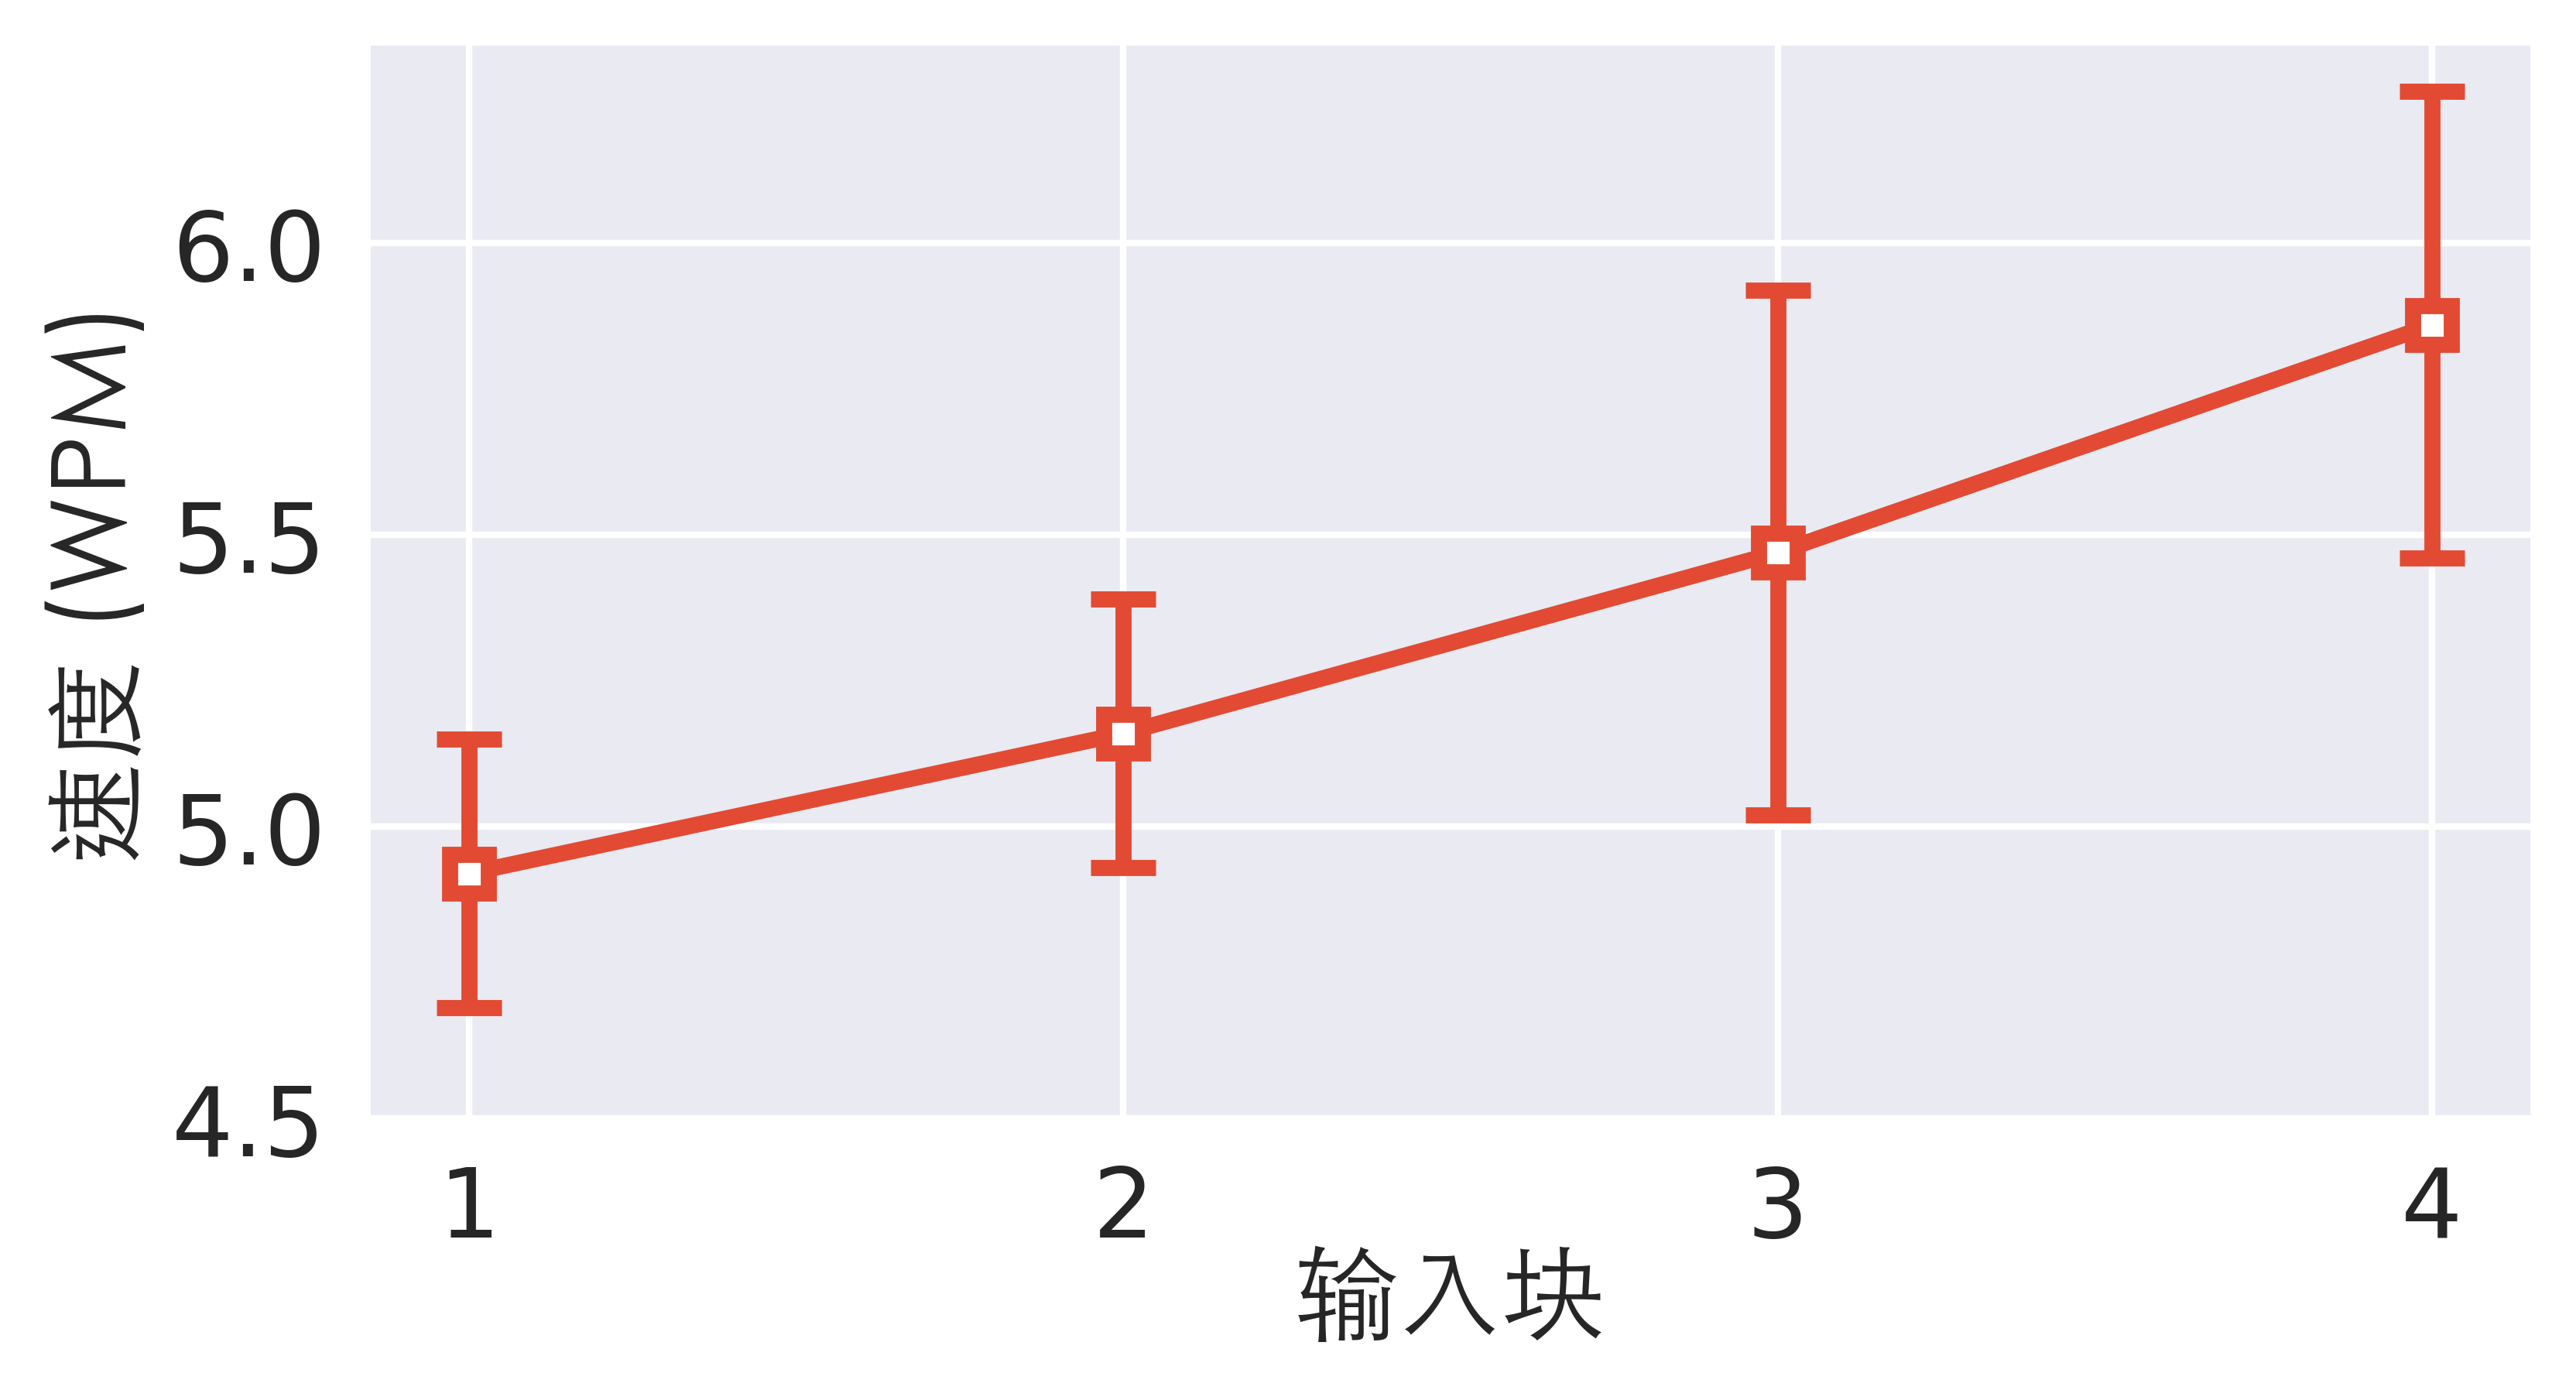
\includegraphics[height=3.5cm]{figures/charspeed.png}}%
  \hspace{4em}%
  \subcaptionbox{字符模式操作次数\label{fig:charops}}
      {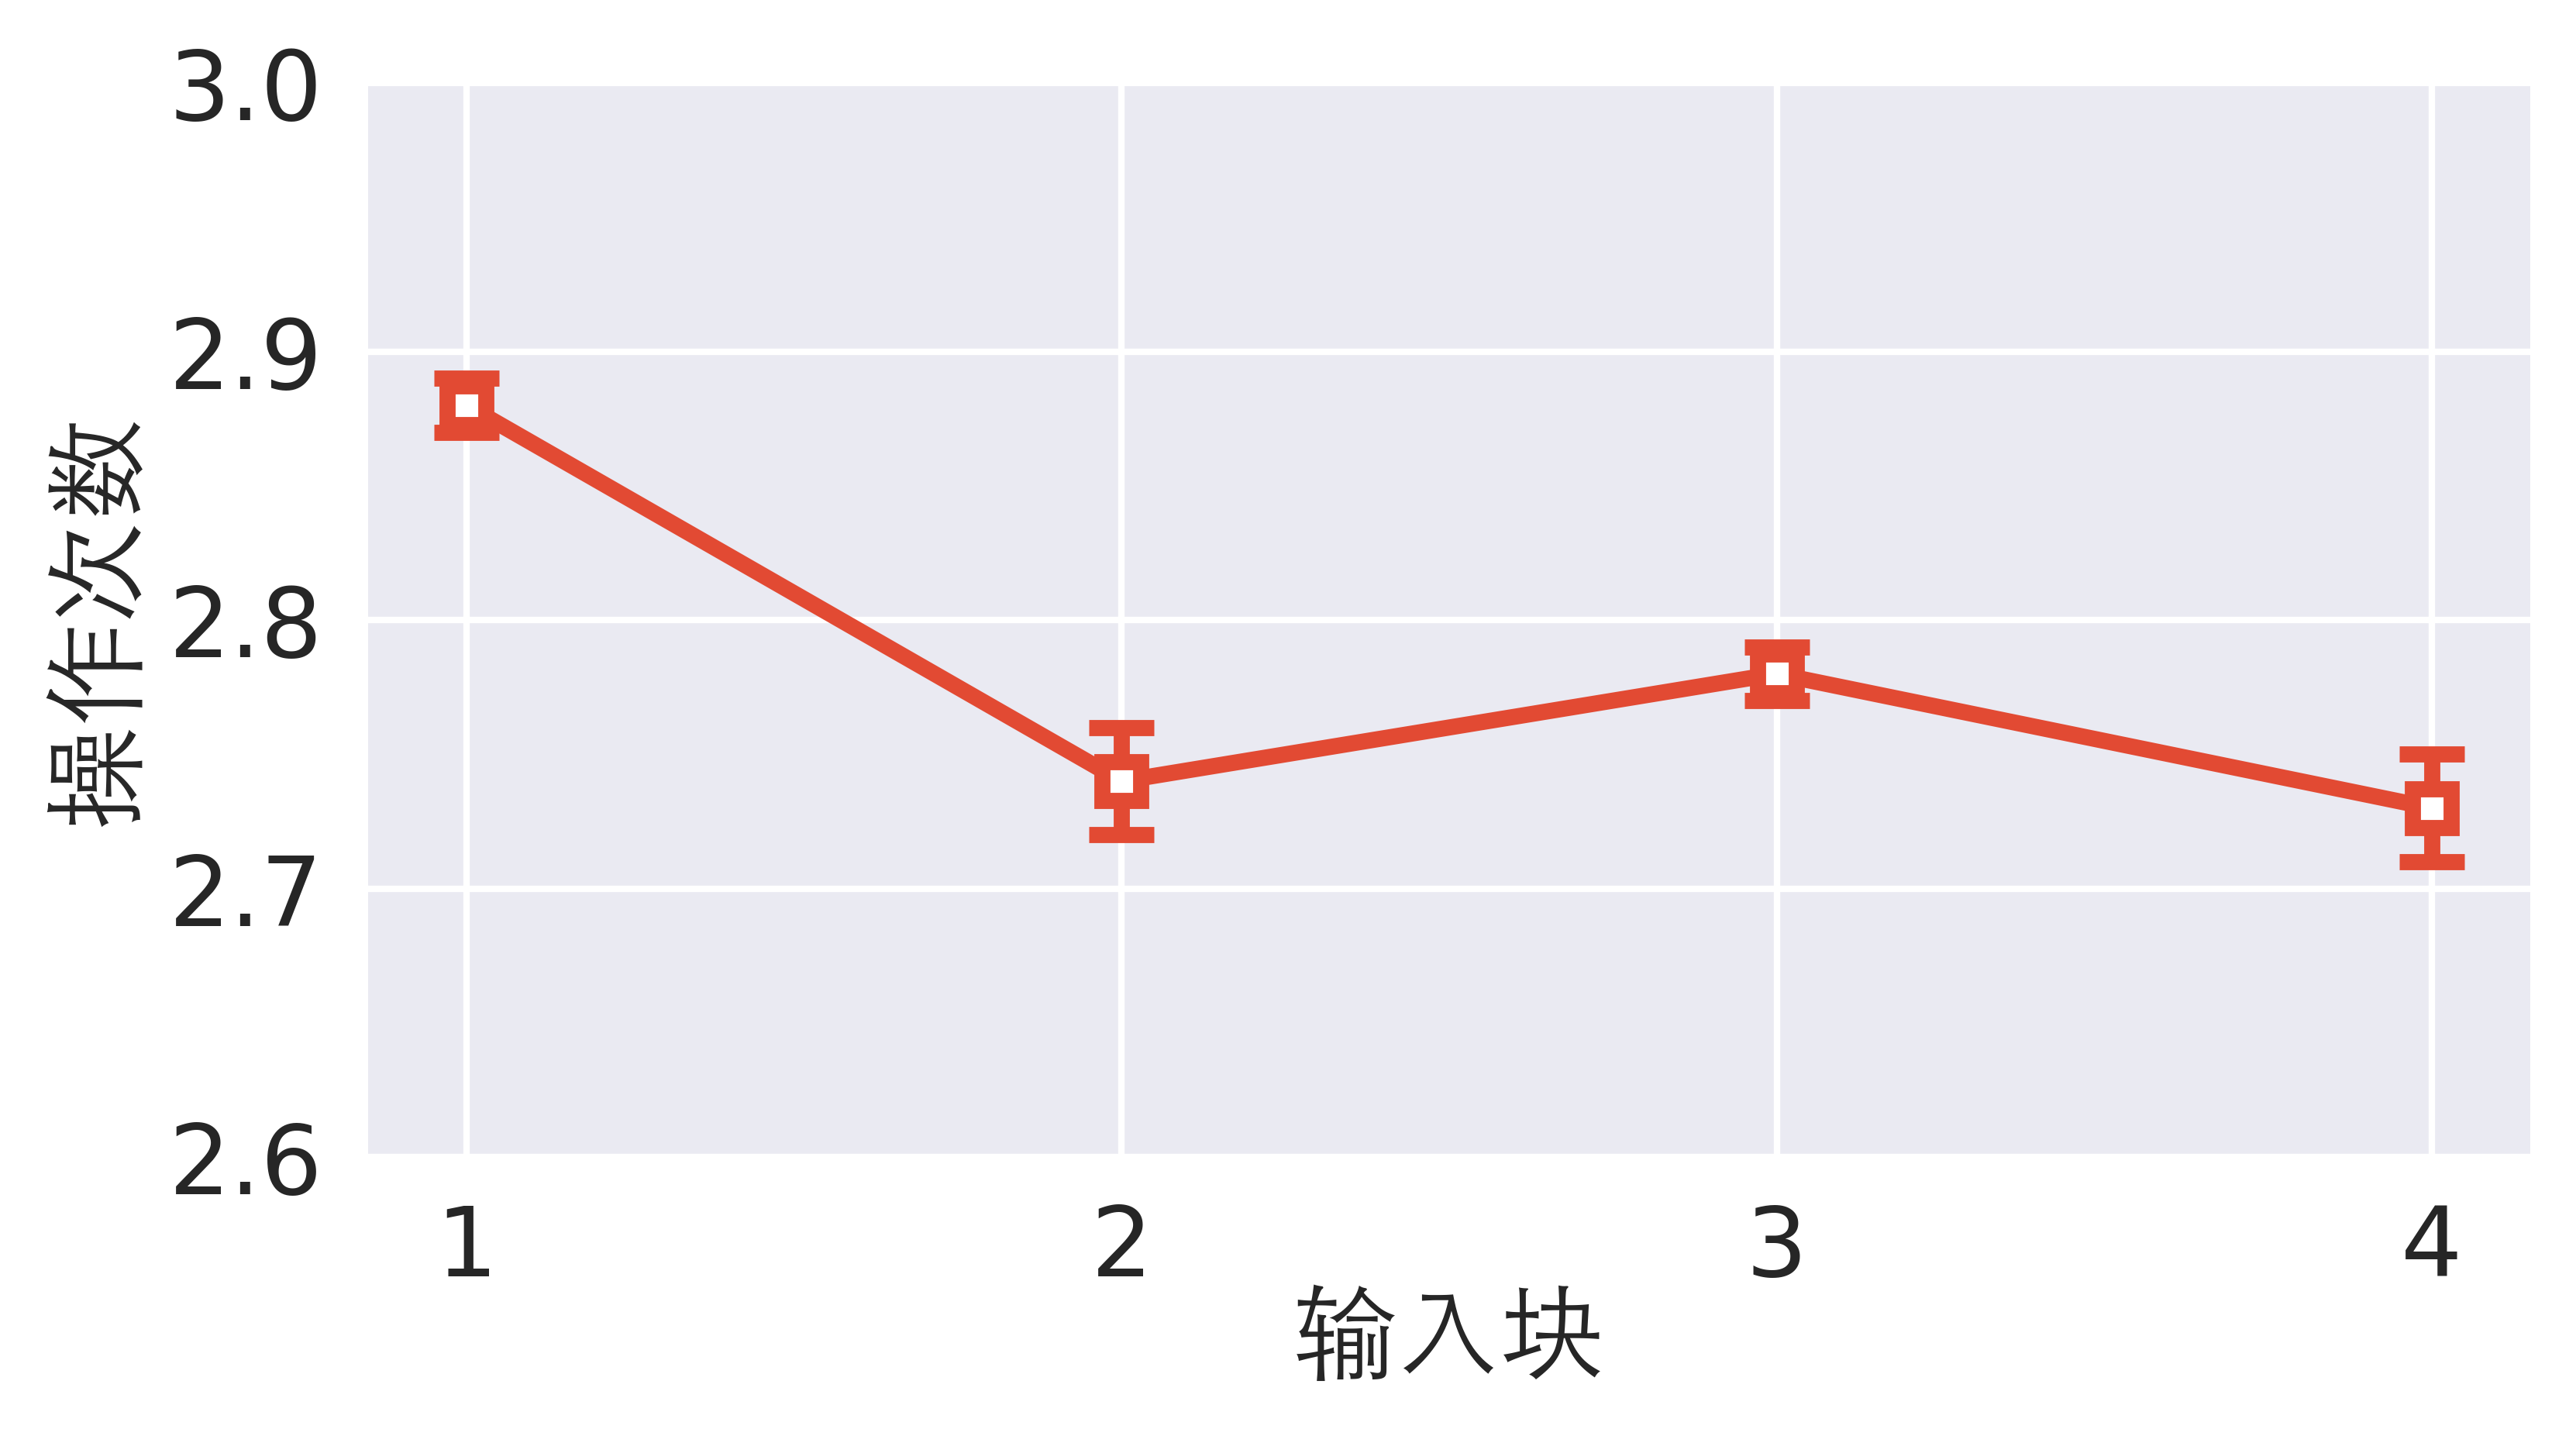
\includegraphics[height=3.5cm]{figures/ops.png}}
  \caption{字符模式速度和操作次数}
  \label{fig:charres}
\end{figure}

字符模式下,平均输入速度为5.36WPM(标准差=0.47),快于手机上控制一维光标或者二维触摸屏划分区域进行输入字符的速度\cite{2018forceboard}\cite{1dhandwriting}。我们还计算了用户每个输入块的平均操作次数,即上滑、左滑右滑次数。操作次数平均为2.68(标准差=0.18)。输入速度和($F_{4,8}=5.06, p < .05$)操作次数($F_{4,8}=36.62, p < .001$)和输入块显著相关,说明用户能够逐渐熟练掌握我们的输入方法,这一点从从图~\ref{fig:charres}也可以看出。

字符模式输入下,输入块和CER关系不显著($F_{4,8}=0.38, p =0.77$),并且CER维持在较低的水平,平均为1.4\%(标准差=1.1\%)。原因在于用户逐个输入字符出错概率较低,即使出错也会重新输入。

\section{单词模式输入}

\subsection{输入速度}
用户在输入单词时的平均速度为40.32WPM(标准差=3.40),输入速度随着输入块增加,在最后一个输入块的平均速度为44.19WPM,该速度与触摸屏上十指盲打基本一致\cite{2018shitoast},慢于在物理键盘上的速度。输入速度和输入块显著相关($F_{4,8}=59.78, p < .001$)。

\subsection{输入准确性}

在单词输入模式中,CER整体平均值为0.37\%(标准差=0.42\%),与输入块的关系不显著($F_{4,8}=2.70, p =0.14$)。总体来看,CER仍然处于较低的水平,原因有两点,一是我们的算法准确性较高,能够预测用户的目标单词;二是即使用户点错位置或者选择了错误的单词,通常会选择重新进行输入。

\subsection{用户行为数据}
我们统计了用户在单词级别输入时的交互数据,其中“单词一匹配”表示用户选择了出现的第一个单词,且该单词与目标句子对应单词相同,“单词一不匹配”则表示选择单词一但是该单词错误;以此类推,“非单词一匹配”和“非单词一不匹配”分别表示用户选择的单词不是第一个时,该单词正确与否的情况。“撤销”操作表示用户未输入完一个单词时清空当前的输入内容;“删除”则表示用户删除输入框中一个单词,一般为选择了错误的单词后删除重新输入。

\begin{table}[h]
  \centering
  \begin{minipage}[t]{0.9\linewidth} % 如果想在表格中使用脚注,minipage是个不错的办法
  \caption[单词模式下用户各行为百分比]{单词模式下用户各行为百分比}
  \label{tab:word-stat}
    \centering
    \begin{tabularx}{\linewidth}{cccccc}
      \toprule[1.5pt]
      %  & \multicolumn{2}{c}{总体}&\multicolumn{2}{c}{左手} &  \multicolumn{2}{c}{右手} \\\midrule[1pt]
      单词一匹配 & 单词一不匹配 & 非单词一匹配 & 非单词一不匹配 & 删除 & 撤销\\\midrule[1pt]
      72.10 & 2.74 & 20.81 & 0.65 & 2.10 & 1.61\\
      \bottomrule[1.5pt]
    \end{tabularx}
  \end{minipage}
\end{table}

从表格~(\ref{tab:word-stat})可以看出,用户的绝大部分操作为“单词一匹配”(72.10\%),说明我们的算法能够很好预测用户的目标单词。不匹配的情况大部分出现在选择单词一时,表示用户输入完成一个单词直接点击确定,造成输入错误,然后用户会将该单词删除重新输入。该行为从侧面反应用户较为熟练我们的使用方法,出现类似在物理键盘上的行为。


\section{混合模式输入} 

\subsection{输入速度}
用户在混合模式下,整体的输入速度为17.63WPM(标准差=1.93),该速度快于智能手表的输入技术\cite{compass},稍慢于手机单手输入\cite{2017blindtype}。然而,这里提到的这两种输入方式都仅为单词输入,而我们在混合模式下输入即能达到该速度,证明了我们技术的实用性。另外,输入单词的平均速度为40.25WPM(标准差=2.80),输入字符的平均速度为5.10WPM(标准差=0.39)。不同输入块差距不明显(输入单词时$F_{4,8}=1.49, p =0.30$,输入字符时$F_{4,8}=0.82, p =0.52$),表明在经过前面两个模式的实验之后,用户较为熟悉了我们的输入方法。在混合模式下,输入单词和字符的速度较单独输入有所下降,说明用户在切换模式时需要一定时间进行调整。

\begin{figure}[h] % use float package if you want it here
    \centering
    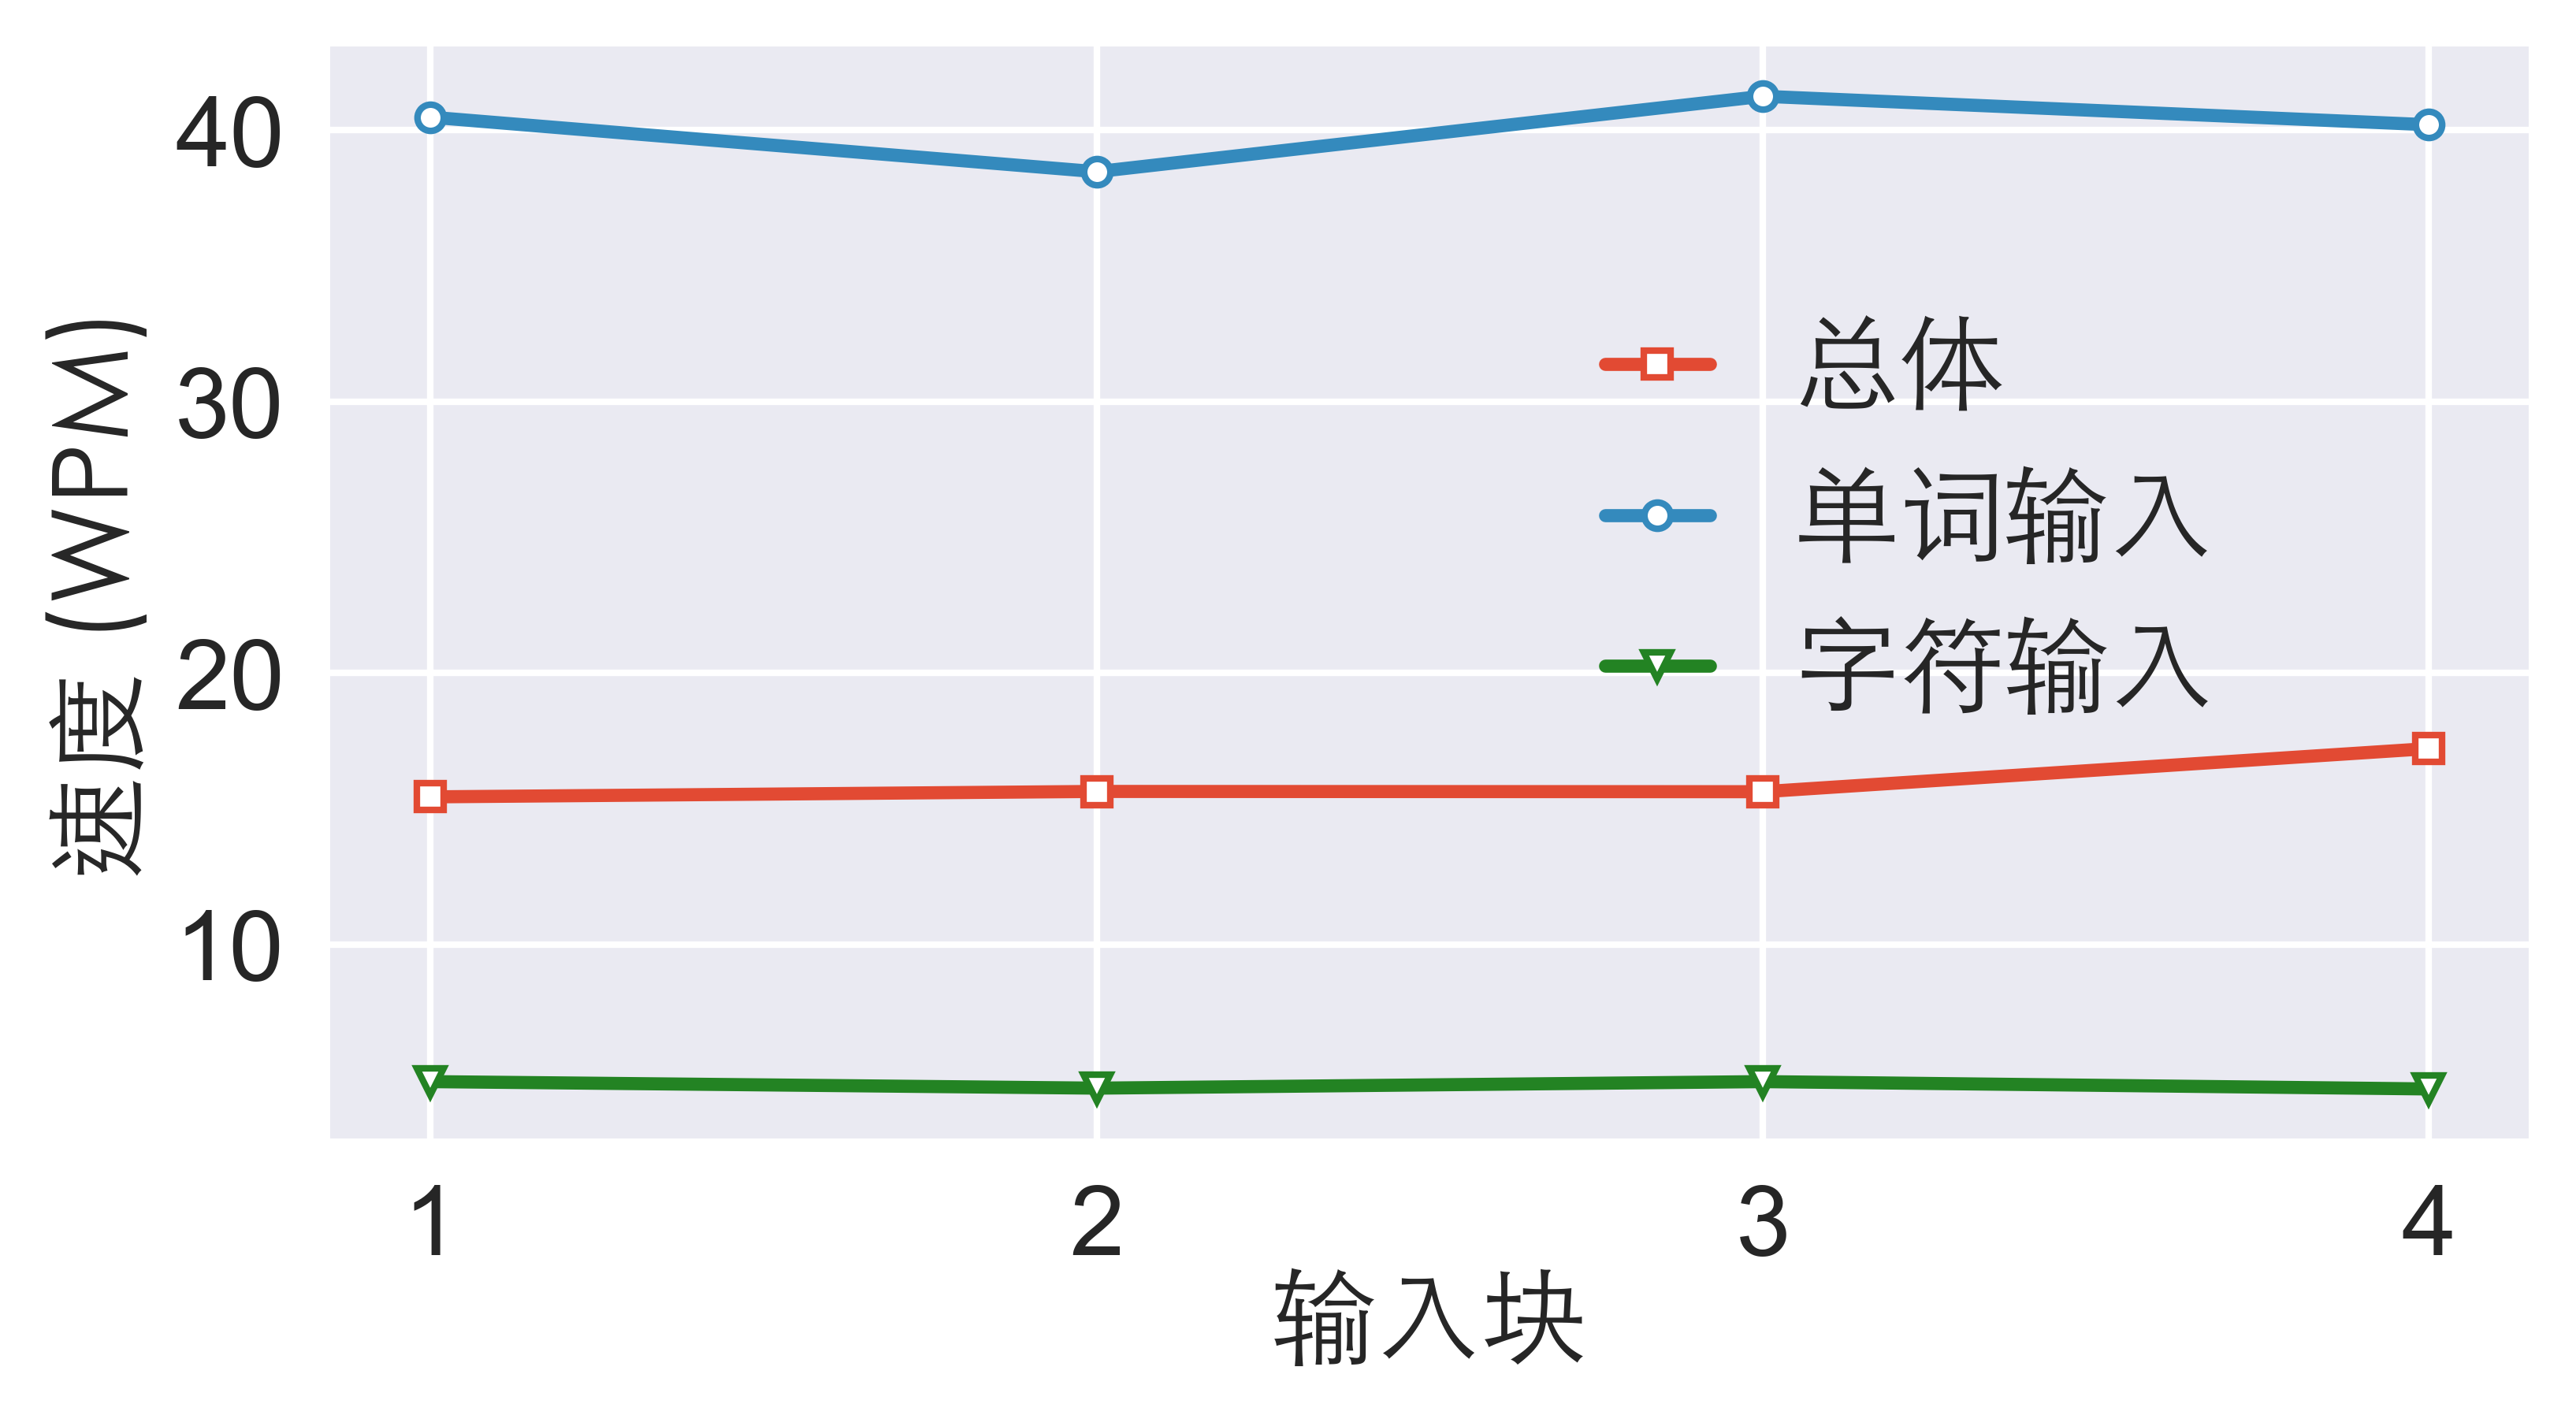
\includegraphics[height=5cm]{figures/wholespeed.png}
    \caption{混合模式输入速度}
    \label{fig:wholespeed}
\end{figure}


\subsection{输入准确性}
用户的输入准确性较高,总体、输入单词、输入字符的CER分别为0.6\%(标准差=0.3\%),0.7\%(标准差=0.6\%),0.9\%(标准差=1.1\%),均与输入块无明显相关性。

\subsection{用户行为数据}
用户在输入字符时的平均操作次数为2.72(标准差=0.21),和单独输入字符时基本一致,说明混合输入对用户输入字符的行为影响不大。操作次数和输入块无明显关联($F_{4,8}=0.91, p =0.48$)。

和单词模式输入相同,我们同样统计了用户在输入单词时的交互行为数据,如表~\ref{tab:hybrid-stat}。“单词一匹配”的百分比有所下降,对应的“非单词一匹配”的百分比上升,说明用户在混合模式下输入准确性有所下降,可能为输入字符前后手的位置有所变化造成了点击准确度降低。

\begin{table}[h]
  \centering
  \begin{minipage}[t]{0.9\linewidth} % 如果想在表格中使用脚注,minipage是个不错的办法
  \caption[混合模式下用户输入单词各行为百分比]{混合模式下用户输入单词各行为百分比}
  \label{tab:hybrid-stat}
    \centering
    \begin{tabularx}{\linewidth}{cccccc}
      \toprule[1.5pt]
      %  & \multicolumn{2}{c}{总体}&\multicolumn{2}{c}{左手} &  \multicolumn{2}{c}{右手} \\\midrule[1pt]
      单词一匹配 & 单词一不匹配 & 非单词一匹配 & 非单词一不匹配 & 删除 & 撤销\\\midrule[1pt]
      69.97 & 3.86 & 24.52 & 0.00 & 1.1 & 0.51\\
      \bottomrule[1.5pt]
    \end{tabularx}
  \end{minipage}
\end{table}

\section{本章总结}
在本章中,我们详细介绍了我们系统的具体实现,并且对提到的三种输入模式分别进行了用户评测。结果表明,使用我们的技术,输入单词的速度能够超过了40WPM,输入字符的速度超过了5WPM,混合输入的速度接近18WPM。同时,输入的准确性也能够得到保证。通过在实际使用场景下的用户实验,我们证明了本输入技术的高效性。

% !TeX root = ../main.tex
\chapter{总结和未来工作}
\label{cha:conclusion}
\section{讨论}

\section{未来工作} %limitation: 声音、图像机器学习、插入删除、支持更好的休息、更多的人
\section{总结}


% 其它部分
\backmatter

%% 本科生要求的几个索引。
\listoffigures    % 插图索引
\listoftables     % 表格索引
\listofequations  % 公式索引

% 参考文献
\bibliographystyle{thuthesis-numeric}      % 顺序编码制
% \bibliographystyle{thuthesis-author-year}  % 著者-出版年制
% \bibliographystyle{thuthesis-bachelor}     % 本科生参考文献的著录格式
\bibliography{ref/refs}

% 致谢
% !TeX root = ../main.tex

\begin{acknowledgements}
  衷心感谢导师陶品老师对我研究的支持。
  
  感谢易鑫老师把我带进人机交互这个领域,您一直以来不厌其烦的指导和帮助是我能够顺利完成一个个项目的关键!您对问题的思考、对研究的热爱为我树立了很好的榜样。同时也要感谢实验室喻老师和史老师的指导。

  感谢我的父亲和母亲21年来对我的关爱和支持。没有你们的牺牲和付出,我也难以进入清华并获得海外深造的机会。感谢我的爷爷奶奶在我童年时期对我的悉心关怀和培养,虽然你们文化程度不高,但是你们用自己的一言一行让我从小就培养了热爱学习这个终身受益的习惯。

  感谢贵系所有老师的谆谆教诲。感谢计65班的李文凯、李映辉等同班同学四年来的相互鼓励和帮助,相信球场上的共同拼搏以及学习上的共同进步这段在清华的时光会成为我们彼此人生中难忘的经历。
\end{acknowledgements}


% 声明
\statement

% 附录
\appendix
% !TeX root = ../main.tex

\begin{survey}
\label{cha:survey}

\title{An Overview on Text Entry Research}
\maketitle

Text Entry refers to the behavior of entering characters into electronic devices such as laptops, mobile phones. Over the last few years, the typing interface has changed a lot, from physical keyboards to virtual keyboards on mobile phones and smartwatches, VR keyboard, etc. Although the evolution of interfaces has greatly facilitated our life, it brings challenges to researchers. Text entry research often focus on four aspects: modeling of user input behavior, touch detection, algorithms and interface design.

\section{User Input Behavior}
User behavior study is the cirtical part of human-computer interaction, definitely text entry not excluded. Users typing behaviors differ a lot in different situations. Findlater\cite{flatglass2011} did a comprehensive study on how expert physical keyboard users typing patterns appeared on touch screens. The study revealed that participants typed with an average of 58.5WPM. In addition, most touches fell within the bounding box of corresponding keys. Even when the keyboard was invisible, the emergent keyboard also showed a QWERTY layout. Therefore, users could transfer their muscle memory of physical keyboards to touch screens. TOAST \cite{shi2018toast} further proved that users' touch points on a large touchable surface also formed a gaussian distribution with QWERTY layout. Furthermore, fitting keyboard location and size tended to drift over time, suggesting the necessity of an adaptive algorithm.

With the increasing popularity of mobile devices, researchers also started exploring mobile text entry behaviors. BlindType\cite{lu2017blindtype} tried to investigate people's eyes-free typing on a touchpad using one thumb. It showed that participants could get familiar with one-thumb eyes-free typing with less than five phrases. At the same time, the emergent keyboard layout was similar to a standard QWERTY layout in a smaller size, suggesting that muscle memory could even be transferred to eyes-free use. Yi \cite{yi2017too} did a user study to test five different keyboard sizes ranging from 2.0cm - 4.0cm, finding that participants could type over 20WPM on 2.0cm keyboard. However, when the keyboard became smaller, the error rate increased significantly. Consistent with other works, the spread of space key was significantly larger compared to normal keys.

\section{Touch Detection}
Touch detection actually depends on what device we use. Capacitive screens are the most widely used sensors for mobile phones and some laptops, such as Microsoft Surface. With a capacitive screen, researchers normally get a 2-dimensional coordinate touch event regarding each tap \cite{shi2018toast, lu2017blindtype}. Force is another commonly used channel, often used to distinguish touches with different characteristics. For example, force can be utilized to choose a letter from ambiguous keyboard in PressureText \cite{mccallum2009pressuretext}, to control the move of cursor in ForceBoard \cite{zhong2018forceboard},.

\section{Algorithms}
Decoding algorithms serve as the role of interpreting user touches, namely, to match either a single tap to a character or a series of taps to a word.

In word-level input, which means we assume users always input word by word, the most commonly used algorithm is based on Na\"ive Bayes devised by Goodman\cite{goodman2002language}. The algorithm aims to find the word with maximum possibility given a sequence of input, which is often an array of 2-dimensional coordinates. The mathematical form can be expressed as follows:
\begin{equation}
  argmax P(W|L) = argmax \frac{P(L|W) \times P(W)}{P(L)}
\end{equation}
in which $L$ is the input letter sequence, $W$ is a word coming from the corpus. Since $P(L)$ stays the same for every word, we can omit calculation. $P(W)$ is the language model that is related to word frequency. By simplicity, we often use bigram language model, that is to consider each tap as independent, which can be calculated by bivariate gaussian distribution. Although simple, it is proved to be very efficient, reducing the error rate by 1.67 - 1.87 in a soft keyboard task \cite{goodman2002language}. 

TOAST \cite{shi2018toast} further proposed a relative decoding algorithm, which was to consider the variation of two consecutive touches together as a Gaussian distribution. This way could reduce the negative effect of hand drifting. Personalized and adaptive algorithms may also be developed for every user.

Depending on specific circumstances, we can also use machine learning algorithms such as Decision Tree, support vector machine to classify different keys.

\section{Interface Design}
Interface design is a comprehensive part that is related to several aspects, including device size, keyboard layout and so on. 

The most common and widely used layout is QWERTY, in both physical and virtual situations. However, QWERTY may not be suitable for certain scenarios. For instance, when the screen is small, QWERTY may cause the "fat finger" problem. Therefore, various forms of layouts came out in response to different needs.

Ambiguous keyboards aim to introduce ambiguity so as to compensate for the inaccuracy of user touches. In ambiguous keyboards, one key would represent more than two or more characters. Each key is also larger, making it easier for people to find and press. T9, standing for Text on 9 keys, is a popular ambiguous keyboard, which can often be found in mobile phones. 1Line Keyboard\cite{li20111line} condensed three rows QWERTY to only one row on iPad, occupying much less space while still remaining 30WPM input speed.

Some keyboards try to make adjustments on QWERTY. Split keyboard, which splits QWERTY by two halves, is often used on tablets when people are holding them. Lu et al. \cite{lu2019typing} improved traditional split keyboard by introducing peripheral typing, which enhanced typing experience with less attention on the keyboard part.

With the development of sensing technologies, some text entry methods without any interface also emerged. Canesta Keyboard \cite{roeber2003typing} enabled typing on any surface by projecting a virtual keyboard via laser. ATK \cite{yi2015atk} introduced a ten-finger eyes-free typing technique in mid-air. With 3-dimensional real-time data, we could track the movement and position of each finger. TipText \cite{xu2019tiptext} even allowed a user to type on his or her tip finger with a thumb finger. The author ran simulations over millions of ambiguous layouts to find the optimal underlying one.

Apart from these, interface design is also related to hand postures. Users can type with ten-fingers, thumbs and one hand.

To sum up, text entry researchers usually focus on the above four aspects. People's typing experience has improved a lot in terms of speed and accuracy. Fast and natural text entry became available in devices like smartwatches. Our work provides possibilities to input text in any feasible flat surface with the signals of mobile phones.

\bibliographystyle{plainnat}
\bibliography{ref/appendix}

\end{survey}
       % 本科生:外文资料的调研阅读报告
% % !TeX root = ../main.tex

\begin{translation}
\label{cha:translation}

\title{书面翻译题目}
\maketitle

\section{单目标规划}
北冥有鱼,其名为鲲。鲲之大,不知其几千里也。化而为鸟,其名为鹏。鹏之背,不知其几
千里也。怒而飞,其翼若垂天之云。是鸟也,海运则将徙于南冥。南冥者,天池也。
\begin{equation}\tag*{(123)}
 p(y|\mathbf{x}) = \frac{p(\mathbf{x},y)}{p(\mathbf{x})}=
\frac{p(\mathbf{x}|y)p(y)}{p(\mathbf{x})}
\end{equation}

吾生也有涯,而知也无涯。以有涯随无涯,殆已!已而为知者,殆而已矣!为善无近名,为
恶无近刑,缘督以为经,可以保身,可以全生,可以养亲,可以尽年。

\subsection{线性规划}
庖丁为文惠君解牛,手之所触,肩之所倚,足之所履,膝之所倚,砉然响然,奏刀騞然,莫
不中音,合于桑林之舞,乃中经首之会。
\begin{table}[ht]
\centering
  \centering
  \caption*{表~1\hskip1em 这是手动编号但不出现在索引中的一个表格例子}
  \label{tab:badtabular3}
  \begin{tabular}[c]{|m{1.5cm}|c|c|c|c|c|c|}\hline
    \multicolumn{2}{|c|}{Network Topology} & \# of nodes &
    \multicolumn{3}{c|}{\# of clients} & Server \\\hline
    GT-ITM & Waxman Transit-Stub & 600 &
    \multirow{2}{2em}{2\%}&
    \multirow{2}{2em}{10\%}&
    \multirow{2}{2em}{50\%}&
    \multirow{2}{1.2in}{Max. Connectivity}\\\cline{1-3}
    \multicolumn{2}{|c|}{Inet-2.1} & 6000 & & & &\\\hline
    \multirow{2}{1.5cm}{Xue} & Rui  & Ni &\multicolumn{4}{c|}{\multirow{2}*{\thuthesis}}\\\cline{2-3}
    & \multicolumn{2}{c|}{ABCDEF} &\multicolumn{4}{c|}{} \\\hline
\end{tabular}
\end{table}

文惠君曰:“嘻,善哉!技盖至此乎?”庖丁释刀对曰:“臣之所好者道也,进乎技矣。始臣之
解牛之时,所见无非全牛者;三年之后,未尝见全牛也;方今之时,臣以神遇而不以目视,
官知止而神欲行。依乎天理,批大郤,导大窾,因其固然。技经肯綮之未尝,而况大坬乎!
良庖岁更刀,割也;族庖月更刀,折也;今臣之刀十九年矣,所解数千牛矣,而刀刃若新发
于硎。彼节者有间而刀刃者无厚,以无厚入有间,恢恢乎其于游刃必有余地矣。是以十九年
而刀刃若新发于硎。虽然,每至于族,吾见其难为,怵然为戒,视为止,行为迟,动刀甚微,
謋然已解,如土委地。提刀而立,为之而四顾,为之踌躇满志,善刀而藏之。”

文惠君曰:“善哉!吾闻庖丁之言,得养生焉。”


\subsection{非线性规划}
孔子与柳下季为友,柳下季之弟名曰盗跖。盗跖从卒九千人,横行天下,侵暴诸侯。穴室枢
户,驱人牛马,取人妇女。贪得忘亲,不顾父母兄弟,不祭先祖。所过之邑,大国守城,小
国入保,万民苦之。孔子谓柳下季曰:“夫为人父者,必能诏其子;为人兄者,必能教其弟。
若父不能诏其子,兄不能教其弟,则无贵父子兄弟之亲矣。今先生,世之才士也,弟为盗
跖,为天下害,而弗能教也,丘窃为先生羞之。丘请为先生往说之。”
\begin{figure}[h]
  \centering
  
\includegraphics{thu-whole-logo.pdf}
  \caption*{图~1\hskip1em 这是手动编号但不出现索引中的图片的例子}
  \label{tab:badfigure3}
\end{figure}

柳下季曰:“先生言为人父者必能诏其子,为人兄者必能教其弟,若子不听父之诏,弟不受
兄之教,虽今先生之辩,将奈之何哉?且跖之为人也,心如涌泉,意如飘风,强足以距敌,
辩足以饰非。顺其心则喜,逆其心则怒,易辱人以言。先生必无往。”

孔子不听,颜回为驭,子贡为右,往见盗跖。

\subsection{整数规划}
盗跖乃方休卒徒大山之阳,脍人肝而餔之。孔子下车而前,见谒者曰:“鲁人孔丘,闻将军
高义,敬再拜谒者。”谒者入通。盗跖闻之大怒,目如明星,发上指冠,曰:“此夫鲁国之
巧伪人孔丘非邪?为我告之:尔作言造语,妄称文、武,冠枝木之冠,带死牛之胁,多辞缪
说,不耕而食,不织而衣,摇唇鼓舌,擅生是非,以迷天下之主,使天下学士不反其本,妄
作孝弟,而侥幸于封侯富贵者也。子之罪大极重,疾走归!不然,我将以子肝益昼餔之膳。”


\nocite{abrahams99tex,salomon1995advanced}
\bibliographystyle{plainnat}
\bibliography{ref/appendix}

% 也可以使用 thebiliography 环境手写
% \begin{thebibliography}{2}
%   \bibitem{abrahams99tex}
%   P.~W. Abrahams, K.~Berry, and K.~A. Hargreaves, \emph{{\TeX} for the
%     Impatient}.\hskip 1em plus 0.5em minus 0.4em\relax Addison-Wesley, 1990.

%   \bibitem{salomon1995advanced}
%   D.~Salomon, ``The advanced {\TeX}book.''\hskip 1em plus 0.5em minus 0.4em\relax
%     New York: Springer, 1995.
% \end{thebibliography}


\end{translation}
  % 本科生:外文资料的书面翻译
% \chapter{单目标规划}

As one of the most widely used techniques in operations
research, \emph{ mathematical programming} is defined as a means of maximizing a
quantity known as \emph{bjective function}, subject to a set of constraints
represented by equations and inequalities. Some known subtopics of mathematical
programming are linear programming, nonlinear programming, multiobjective
programming, goal programming, dynamic programming, and multilevel
programming.

It is impossible to cover in a single chapter every concept of mathematical
programming. This chapter introduces only the basic concepts and techniques of
mathematical programming such that readers gain an understanding of them
throughout the book.


\section{Single-Objective Programming}
The general form of single-objective programming (SOP) is written
as follows,
\begin{equation*} % 如果附录中的公式不想让它出现在公式索引中,那就请
                             % 用 equation*
\left\{\begin{array}{l}
\max \,\,f(x)\\[0.1 cm]
\mbox{subject to:} \\ [0.1 cm]
\qquad g_j(x)\le 0,\quad j=1,2,\cdots,p
\end{array}\right.
\end{equation*}
which maximizes a real-valued function $f$ of
$x=(x_1,x_2,\cdots,x_n)$ subject to a set of constraints.

\newcommand\Real{\mathbf{R}}
\newtheorem{mpdef}{Definition}[chapter]
\begin{mpdef}
In SOP, we call $x$ a decision vector, and
$x_1,x_2,\cdots,x_n$ decision variables. The function
$f$ is called the objective function. The set
\begin{equation*}
S=\left\{x\in\Real^n\bigm|g_j(x)\le 0,\,j=1,2,\cdots,p\right\}
\end{equation*}
is called the feasible set. An element $x$ in $S$ is called a
feasible solution.
\end{mpdef}

\newtheorem{mpdefop}[mpdef]{Definition}
\begin{mpdefop}
A feasible solution $x^*$ is called the optimal
solution of SOP if and only if
\begin{equation}
f(x^*)\ge f(x)
\end{equation}
for any feasible solution $x$.
\end{mpdefop}

One of the outstanding contributions to mathematical programming was known as
the Kuhn-Tucker conditions\ref{eq:ktc}. In order to introduce them, let us give
some definitions. An inequality constraint $g_j(x)\le 0$ is said to be active at
a point $x^*$ if $g_j(x^*)=0$. A point $x^*$ satisfying $g_j(x^*)\le 0$ is said
to be regular if the gradient vectors $\nabla g_j(x)$ of all active constraints
are linearly independent.

Let $x^*$ be a regular point of the constraints of SOP and assume that all the
functions $f(x)$ and $g_j(x),j=1,2,\cdots,p$ are differentiable. If $x^*$ is a
local optimal solution, then there exist Lagrange multipliers
$\lambda_j,j=1,2,\cdots,p$ such that the following Kuhn-Tucker conditions hold,
\begin{equation}
\label{eq:ktc}
\left\{\begin{array}{l}
    \nabla f(x^*)-\sum\limits_{j=1}^p\lambda_j\nabla g_j(x^*)=0\\[0.3cm]
    \lambda_jg_j(x^*)=0,\quad j=1,2,\cdots,p\\[0.2cm]
    \lambda_j\ge 0,\quad j=1,2,\cdots,p.
\end{array}\right.
\end{equation}
If all the functions $f(x)$ and $g_j(x),j=1,2,\cdots,p$ are convex and
differentiable, and the point $x^*$ satisfies the Kuhn-Tucker conditions
(\ref{eq:ktc}), then it has been proved that the point $x^*$ is a global optimal
solution of SOP.

\subsection{Linear Programming}
\label{sec:lp}

If the functions $f(x),g_j(x),j=1,2,\cdots,p$ are all linear, then SOP is called
a {\em linear programming}.

The feasible set of linear is always convex. A point $x$ is called an extreme
point of convex set $S$ if $x\in S$ and $x$ cannot be expressed as a convex
combination of two points in $S$. It has been shown that the optimal solution to
linear programming corresponds to an extreme point of its feasible set provided
that the feasible set $S$ is bounded. This fact is the basis of the {\em simplex
  algorithm} which was developed by Dantzig as a very efficient method for
solving linear programming.
\begin{table}[ht]
\centering
  \centering
  \caption*{Table~1\hskip1em This is an example for manually numbered table, which
    would not appear in the list of tables}
  \label{tab:badtabular2}
  \begin{tabular}[c]{|m{1.5cm}|c|c|c|c|c|c|}\hline
    \multicolumn{2}{|c|}{Network Topology} & \# of nodes &
    \multicolumn{3}{c|}{\# of clients} & Server \\\hline
    GT-ITM & Waxman Transit-Stub & 600 &
    \multirow{2}{2em}{2\%}&
    \multirow{2}{2em}{10\%}&
    \multirow{2}{2em}{50\%}&
    \multirow{2}{1.2in}{Max. Connectivity}\\\cline{1-3}
    \multicolumn{2}{|c|}{Inet-2.1} & 6000 & & & &\\\hline
    \multirow{2}{1.5cm}{Xue} & Rui  & Ni &\multicolumn{4}{c|}{\multirow{2}*{\thuthesis}}\\\cline{2-3}
    & \multicolumn{2}{c|}{ABCDEF} &\multicolumn{4}{c|}{} \\\hline
\end{tabular}
\end{table}

Roughly speaking, the simplex algorithm examines only the extreme points of the
feasible set, rather than all feasible points. At first, the simplex algorithm
selects an extreme point as the initial point. The successive extreme point is
selected so as to improve the objective function value. The procedure is
repeated until no improvement in objective function value can be made. The last
extreme point is the optimal solution.

\subsection{Nonlinear Programming}

If at least one of the functions $f(x),g_j(x),j=1,2,\cdots,p$ is nonlinear, then
SOP is called a {\em nonlinear programming}.

A large number of classical optimization methods have been developed to treat
special-structural nonlinear programming based on the mathematical theory
concerned with analyzing the structure of problems.
\begin{figure}[h]
  \centering
  
\includegraphics{thu-lib-logo.pdf}
  \caption*{Figure~1\quad This is an example for manually numbered figure,
    which would not appear in the list of figures}
  \label{tab:badfigure2}
\end{figure}

Now we consider a nonlinear programming which is confronted solely with
maximizing a real-valued function with domain $\Real^n$.  Whether derivatives are
available or not, the usual strategy is first to select a point in $\Real^n$ which
is thought to be the most likely place where the maximum exists. If there is no
information available on which to base such a selection, a point is chosen at
random. From this first point an attempt is made to construct a sequence of
points, each of which yields an improved objective function value over its
predecessor. The next point to be added to the sequence is chosen by analyzing
the behavior of the function at the previous points. This construction continues
until some termination criterion is met. Methods based upon this strategy are
called {\em ascent methods}, which can be classified as {\em direct methods},
{\em gradient methods}, and {\em Hessian methods} according to the information
about the behavior of objective function $f$. Direct methods require only that
the function can be evaluated at each point. Gradient methods require the
evaluation of first derivatives of $f$. Hessian methods require the evaluation
of second derivatives. In fact, there is no superior method for all
problems. The efficiency of a method is very much dependent upon the objective
function.

\subsection{Integer Programming}

{\em Integer programming} is a special mathematical programming in which all of
the variables are assumed to be only integer values. When there are not only
integer variables but also conventional continuous variables, we call it {\em
  mixed integer programming}. If all the variables are assumed either 0 or 1,
then the problem is termed a {\em zero-one programming}. Although integer
programming can be solved by an {\em exhaustive enumeration} theoretically, it
is impractical to solve realistically sized integer programming problems. The
most successful algorithm so far found to solve integer programming is called
the {\em branch-and-bound enumeration} developed by Balas (1965) and Dakin
(1965). The other technique to integer programming is the {\em cutting plane
  method} developed by Gomory (1959).

\hfill\textit{Uncertain Programming\/}\quad(\textsl{BaoDing Liu, 2006.2})

\section{单目标规划}
北冥有鱼,其名为鲲。鲲之大,不知其几千里也。化而为鸟,其名为鹏。鹏之背,不知其几
千里也。怒而飞,其翼若垂天之云。是鸟也,海运则将徙于南冥。南冥者,天池也。
\begin{equation}\tag*{(123)}
 p(y|\mathbf{x}) = \frac{p(\mathbf{x},y)}{p(\mathbf{x})}=
\frac{p(\mathbf{x}|y)p(y)}{p(\mathbf{x})}
\end{equation}

吾生也有涯,而知也无涯。以有涯随无涯,殆已!已而为知者,殆而已矣!为善无近名,为
恶无近刑,缘督以为经,可以保身,可以全生,可以养亲,可以尽年。

\subsection{线性规划}
庖丁为文惠君解牛,手之所触,肩之所倚,足之所履,膝之所倚,砉然响然,奏刀騞然,莫
不中音,合于桑林之舞,乃中经首之会。
\begin{table}[ht]
\centering
  \centering
  \caption*{表~1\hskip1em 这是手动编号但不出现在索引中的一个表格例子}
  \label{tab:badtabular3}
  \begin{tabular}[c]{|m{1.5cm}|c|c|c|c|c|c|}\hline
    \multicolumn{2}{|c|}{Network Topology} & \# of nodes &
    \multicolumn{3}{c|}{\# of clients} & Server \\\hline
    GT-ITM & Waxman Transit-Stub & 600 &
    \multirow{2}{2em}{2\%}&
    \multirow{2}{2em}{10\%}&
    \multirow{2}{2em}{50\%}&
    \multirow{2}{1.2in}{Max. Connectivity}\\\cline{1-3}
    \multicolumn{2}{|c|}{Inet-2.1} & 6000 & & & &\\\hline
    \multirow{2}{1.5cm}{Xue} & Rui  & Ni &\multicolumn{4}{c|}{\multirow{2}*{\thuthesis}}\\\cline{2-3}
    & \multicolumn{2}{c|}{ABCDEF} &\multicolumn{4}{c|}{} \\\hline
\end{tabular}
\end{table}

文惠君曰:“嘻,善哉!技盖至此乎?”庖丁释刀对曰:“臣之所好者道也,进乎技矣。始臣之
解牛之时,所见无非全牛者;三年之后,未尝见全牛也;方今之时,臣以神遇而不以目视,
官知止而神欲行。依乎天理,批大郤,导大窾,因其固然。技经肯綮之未尝,而况大坬乎!
良庖岁更刀,割也;族庖月更刀,折也;今臣之刀十九年矣,所解数千牛矣,而刀刃若新发
于硎。彼节者有间而刀刃者无厚,以无厚入有间,恢恢乎其于游刃必有余地矣。是以十九年
而刀刃若新发于硎。虽然,每至于族,吾见其难为,怵然为戒,视为止,行为迟,动刀甚微,
謋然已解,如土委地。提刀而立,为之而四顾,为之踌躇满志,善刀而藏之。”

文惠君曰:“善哉!吾闻庖丁之言,得养生焉。”


\subsection{非线性规划}
孔子与柳下季为友,柳下季之弟名曰盗跖。盗跖从卒九千人,横行天下,侵暴诸侯。穴室枢
户,驱人牛马,取人妇女。贪得忘亲,不顾父母兄弟,不祭先祖。所过之邑,大国守城,小
国入保,万民苦之。孔子谓柳下季曰:“夫为人父者,必能诏其子;为人兄者,必能教其弟。
若父不能诏其子,兄不能教其弟,则无贵父子兄弟之亲矣。今先生,世之才士也,弟为盗
跖,为天下害,而弗能教也,丘窃为先生羞之。丘请为先生往说之。”
\begin{figure}[h]
  \centering
  
\includegraphics{thu-whole-logo.pdf}
  \caption*{图~1\hskip1em 这是手动编号但不出现索引中的图片的例子}
  \label{tab:badfigure3}
\end{figure}

柳下季曰:“先生言为人父者必能诏其子,为人兄者必能教其弟,若子不听父之诏,弟不受
兄之教,虽今先生之辩,将奈之何哉?且跖之为人也,心如涌泉,意如飘风,强足以距敌,
辩足以饰非。顺其心则喜,逆其心则怒,易辱人以言。先生必无往。”

孔子不听,颜回为驭,子贡为右,往见盗跖。

\subsection{整数规划}
盗跖乃方休卒徒大山之阳,脍人肝而餔之。孔子下车而前,见谒者曰:“鲁人孔丘,闻将军
高义,敬再拜谒者。”谒者入通。盗跖闻之大怒,目如明星,发上指冠,曰:“此夫鲁国之
巧伪人孔丘非邪?为我告之:尔作言造语,妄称文、武,冠枝木之冠,带死牛之胁,多辞缪
说,不耕而食,不织而衣,摇唇鼓舌,擅生是非,以迷天下之主,使天下学士不反其本,妄
作孝弟,而侥幸于封侯富贵者也。子之罪大极重,疾走归!不然,我将以子肝益昼餔之膳。”


% 个人简历
% !TeX root = ../main.tex

\begin{resume}

  \resumeitem{个人简历}

  1999 年 05 月 30 日出生于 安徽 省 庐江 县。

  2016 年 8 月考入 清华 大学 计算机科学与技术 系 计算机科学与技术 专业,攻读学士学位至今。
  % ,xxxx 年 7 月本科毕业并获得 xx 学士学位。

  % xxxx 年 9 月免试进入 xx 大学 xx 系攻读 xx 学位至今。

  \researchitem{发表的学术论文} % 发表的和录用的合在一起

  % 1. 已经刊载的学术论文(本人是第一作者,或者导师为第一作者本人是第二作者)
  \begin{publications}
    \item Xin Yi, \textbf{Chen Wang}, Xiaojun Bi, Yuanchun Shi. 2020. PalmBoard: Leveraging Implicit Touch Pressure in Statistical Decoding for Indirect Text Entry (CHI' 20). ACM, Honolulu, HI, USA, Paper 314, 13 pages. https://doi.org/10.1145/3313831.3376441
    % \item 杨轶, 张宁欣, 任天令, 等. 硅基铁电微声学器件中薄膜残余应力的研究. 中国机
    %   械工程, 2005, 16(14):1289-1291. (EI 收录, 检索号:0534931 2907.)
    % \item 杨轶, 张宁欣, 任天令, 等. 集成铁电器件中的关键工艺研究. 仪器仪表学报,
    %   2003, 24(S4):192-193. (EI 源刊.)
  \end{publications}

  % % 2. 尚未刊载,但已经接到正式录用函的学术论文(本人为第一作者,或者
  % %    导师为第一作者本人是第二作者)。
  % \begin{publications}[before=\publicationskip,after=\publicationskip]
  %   \item Yang Y, Ren T L, Zhu Y P, et al. PMUTs for handwriting recognition. In
  %     press. (已被 Integrated Ferroelectrics 录用. SCI 源刊.)
  % \end{publications}

  % % 3. 其他学术论文。可列出除上述两种情况以外的其他学术论文,但必须是
  % %    已经刊载或者收到正式录用函的论文。
  % \begin{publications}
  %   \item Wu X M, Yang Y, Cai J, et al. Measurements of ferroelectric MEMS
  %     microphones. Integrated Ferroelectrics, 2005, 69:417-429. (SCI 收录, 检索号
  %     :896KM)
  %   \item 贾泽, 杨轶, 陈兢, 等. 用于压电和电容微麦克风的体硅腐蚀相关研究. 压电与声
  %     光, 2006, 28(1):117-119. (EI 收录, 检索号:06129773469)
  %   \item 伍晓明, 杨轶, 张宁欣, 等. 基于MEMS技术的集成铁电硅微麦克风. 中国集成电路,
  %     2003, 53:59-61.
  % \end{publications}

  % \researchitem{研究成果} % 有就写,没有就删除
  % \begin{achievements}
  %   \item 任天令, 杨轶, 朱一平, 等. 硅基铁电微声学传感器畴极化区域控制和电极连接的
  %     方法: 中国, CN1602118A. (中国专利公开号)
  %   \item Ren T L, Yang Y, Zhu Y P, et al. Piezoelectric micro acoustic sensor
  %     based on ferroelectric materials: USA, No.11/215, 102. (美国发明专利申请号)
  % \end{achievements}

\end{resume}


% 本科生的综合论文训练记录表
% 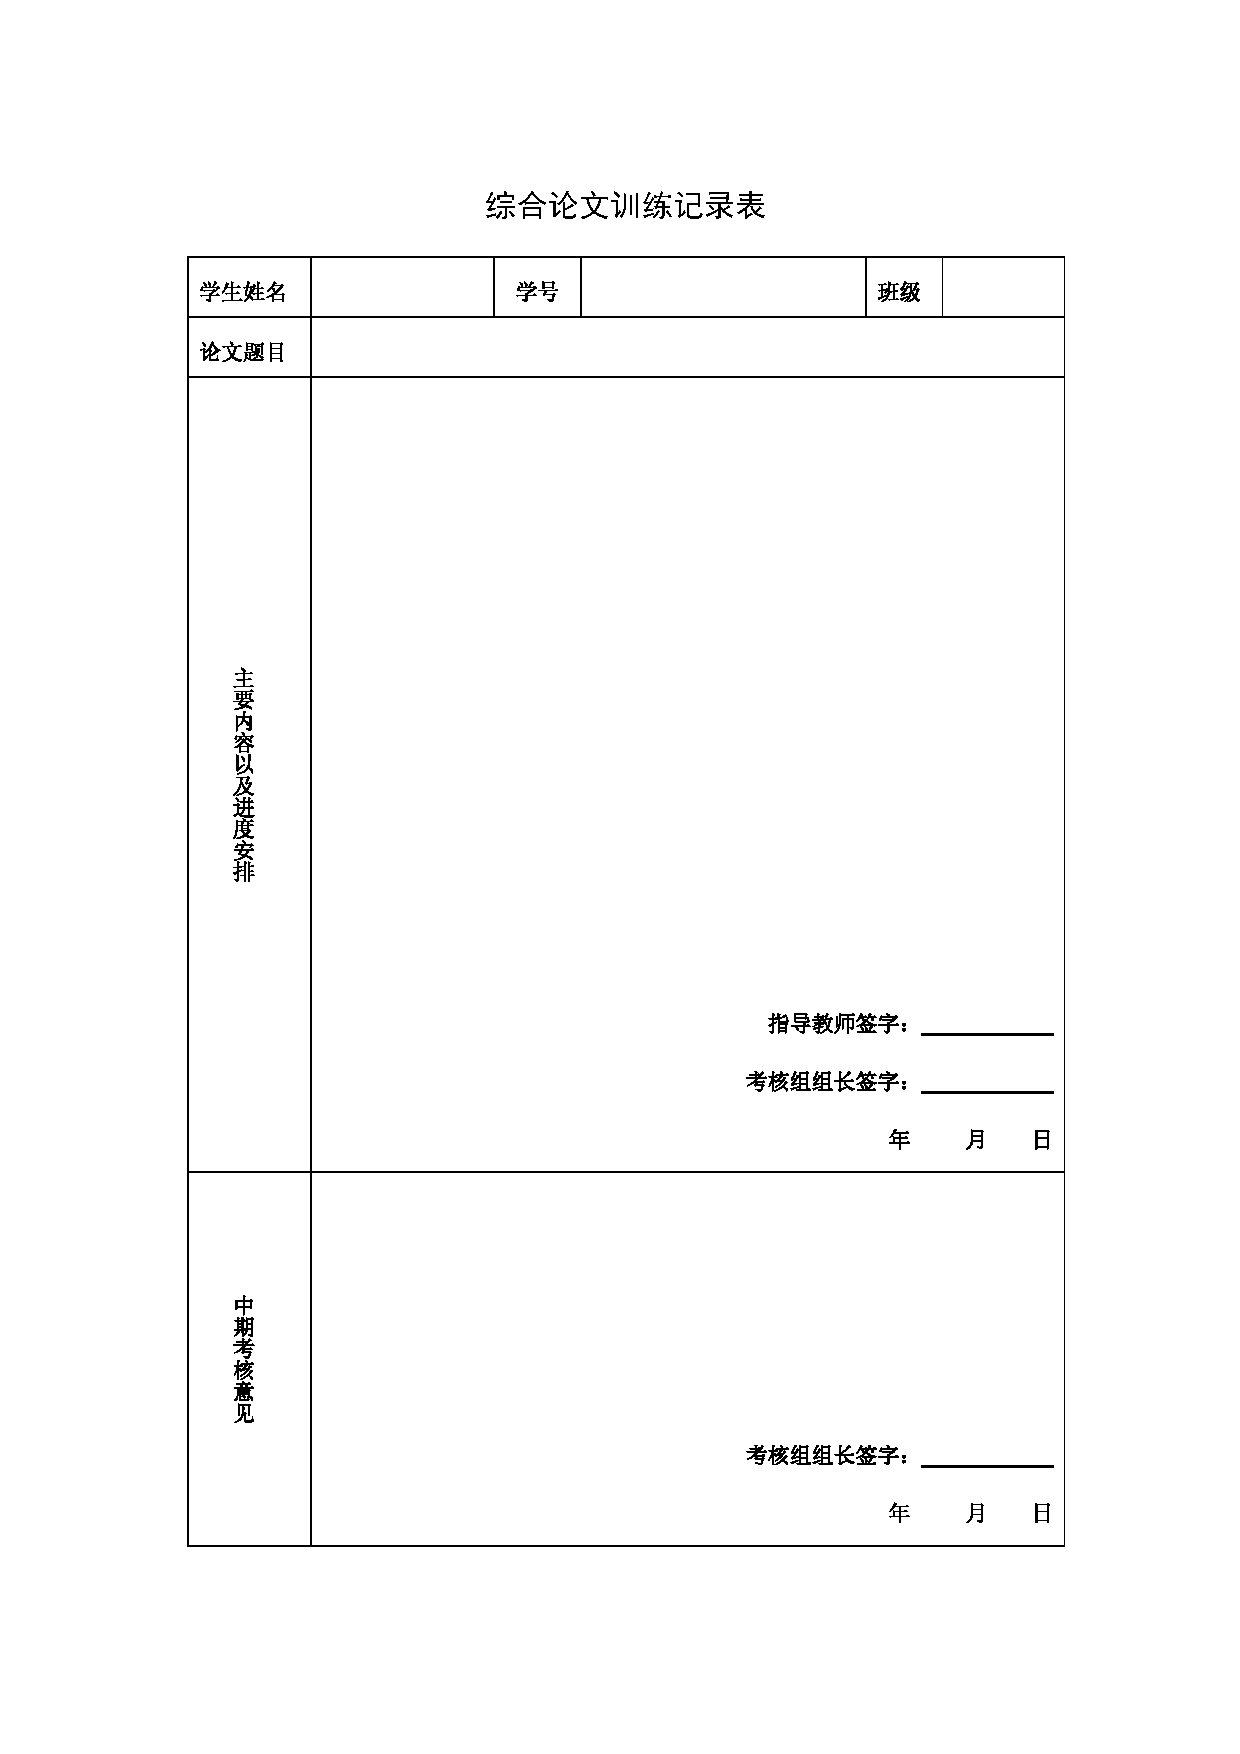
\includepdf[pages=-]{scan-record.pdf}

\end{document}
